\documentclass[a4paper,12pt]{article}
\usepackage[utf8]{inputenc}
\usepackage{graphicx}
\usepackage{float}%"Плавающие" картинки
\usepackage{wrapfig}%Обтекание фигур (таблиц, картинок и прочего)
\usepackage{amsmath, amssymb, amsthm}
\usepackage[T1, T2A]{fontenc}
\usepackage[english, russian]{babel}
\usepackage[left=1cm,right=1cm, top=1cm, bottom=2cm]{geometry}
% Межстрочный интервал = 1.5pt
\usepackage{setspace}
\onehalfspacing
% % Абзацный отступ = 1.25см
%\usepackage{indentfirst}
%\setlength\parindent{0mm}
% Путь до папки с изображениями
\graphicspath{ {../img/} }
% listings
\usepackage{minted}
% Активные ссылки на формулы и лит-ру
\usepackage[
  colorlinks=true,
  citecolor=blue,
  linkcolor=blue,
  linktoc=page,
]{hyperref}
\usepackage[all]{hypcap}
\usepackage{makecell}

% cleverref
\usepackage{cleveref}
\newcommand{\crefrangeconjunction}{~--~}
\newcommand{\crefpairconjunction}{, }
\newcommand{\creflastconjunction}{, }
\crefname{equation}{}{}

% enumeration
\numberwithin{equation}{section}

\usepackage{xcolor}
\usepackage{mdframed}
\usepackage{cancel}
\newcommand{\Ren}{\mathrm{Re}}
\newcommand{\Pen}{\mathrm{Pe}}
\newcommand{\Nun}{\mathrm{Nu}}
\renewcommand{\vec}[1]{\boldsymbol{\rm #1}}
\newcommand{\dfr}[2]{\frac{\partial #1}{\partial #2}}
\newcommand{\dfrq}[2]{\frac{\partial^2 #1}{\partial #2^2}}
\newcommand{\ddfr}[2]{\dfrac{\partial #1}{\partial #2}}
\newcommand{\ddfrq}[2]{\dfrac{\partial^2 #1}{\partial #2^2}}
\newcommand{\sfrac}[2]{\left.#1\middle/#2\right.}
\newcommand{\dsfr}[2]{\left.\partial #1\middle/\partial#2\right.}
\newcommand{\FL}[2]{#1\cdot10^{#2}}
\newcommand{\eps}{\varepsilon}
\newcommand{\hence}{\quad\Rightarrow\quad}
\newcommand{\imi}{\mathbf{i}}
\newcommand{\upx}[1]{{\mathrm{upx}\left[#1\right]}}
\newcommand{\upy}[1]{{\mathrm{upy}\left[#1\right]}}
\definecolor{ename-color}{rgb}{0.9, 0.9, 0.9}
\newcommand\lword[1]{\leavevmode\nobreak\hskip0pt plus\linewidth\penalty50\hskip0pt plus-\linewidth\nobreak#1}
\newcommand{\ename}[1]{\lword\colorbox{ename-color}{\Verb!#1!}}
\newcommand{\cvar}[1]{\lword\mintinline{text}{#1}}
\newcommand{\figref}[1]{рис.~\ref{#1}}
\newenvironment{shelloutput}%
  {\VerbatimEnvironment
    \begin{mdframed}[backgroundcolor=beige]
    \begin{Verbatim}}
  {\end{Verbatim}%
    \end{mdframed}}
\newcommand{\dt}{\triangle t}
\newcommand{\pluseq}{{{+}{=}}}
\newcommand{\minuseq}{{{-}{=}}}
\newcommand{\multeq}{{{*}{=}}}
\newcommand{\arint}[3]{\displaystyle\int\limits_{#2}#1 \, d #3}
\newcommand\vecangle[2]{
  \setbox0=\hbox{$\!\vec{#1},\vec{#2}\!$}
  \ht0=\dimexpr\ht0-1pt\relax
  \widehat{\copy0}\,
}
\newcommand{\gvec}[1]{\left\{#1\right\}}
\newcommand{\quo}[1]{``#1''}
\newcommand{\const}{{\rm const}}
\newcommand{\mat}[1]{{\rm #1}}

\usepackage{pythontex}
\usepackage{minted}
\definecolor{beige}{rgb}{0.96, 0.96, 0.86}

\setminted{
        bgcolor=beige,
        linenos,
        xleftmargin=0pt,
        breaklines=true,
        numbersep=2pt,
        tabsize=2
    }

\begin{pycode}
from clisting import *
\end{pycode}

\newcommand{\clisting}[2]{\pyc{clisting_func("#1", #2)}}

\newenvironment{cppcode}
  {
    \VerbatimEnvironment%
    \begin{minted}[linenos=false]{c++}%
  }
  {
    \end{minted}%
  }

\usepackage{titlesec}

\titleclass{\subsubsubsection}{straight}[\subsection]

\newcounter{subsubsubsection}[subsubsection]
\renewcommand\thesubsubsubsection{\thesubsubsection.\arabic{subsubsubsection}}
\renewcommand\theparagraph{\thesubsubsubsection.\arabic{paragraph}} % optional; useful if paragraphs are to be numbered

\titleformat{\subsubsubsection}
  {\normalfont\normalsize\bfseries}{\thesubsubsubsection}{1em}{}
\titlespacing*{\subsubsubsection}
{0pt}{3.25ex plus 1ex minus .2ex}{1.5ex plus .2ex}

\makeatletter
\renewcommand\paragraph{\@startsection{paragraph}{5}{\z@}%
  {3.25ex \@plus1ex \@minus.2ex}%
  {-1em}%
  {\normalfont\normalsize\bfseries}}
\renewcommand\subparagraph{\@startsection{subparagraph}{6}{\parindent}%
  {3.25ex \@plus1ex \@minus .2ex}%
  {-1em}%
  {\normalfont\normalsize\bfseries}}
\def\toclevel@subsubsubsection{4}
\def\toclevel@paragraph{5}
\def\toclevel@paragraph{6}
\def\l@subsubsubsection{\@dottedtocline{4}{7em}{4em}}
\def\l@paragraph{\@dottedtocline{5}{10em}{5em}}
\def\l@subparagraph{\@dottedtocline{6}{14em}{6em}}
\makeatother

\setcounter{secnumdepth}{4}
\setcounter{tocdepth}{4}


\begin{document}

\newpage
\tableofcontents
\newpage

\section{Лекция 1 (02.09)}


\appendix
\section{Формулы и обозначения}
\subsection{Векторы}

\subsubsection{Обозначение}

Геометрические вектора обозначаются жирным шрифтом $\vec v$.
Скалярные координаты вектора -- через нижний индекс с обозначением
оси координат: $\left(v_x, v_y, v_z\right)$.
Если вектор $\vec u$ -- вектор скорости, то его декартовые координаты
имеют специальное обозначение $\vec u = \left(u, v, w\right)$.
Единичные вектора, соответствующие осям координат, обозначаются 
знаком $\hat\cdot$: $\vec{\hat x}$, $\vec{\hat y}$, $\vec{\hat z}$.
Координатные векторы обозначаются по символу первой оси. Например, $\vec x = (x, y, z)$ или $\vec \xi = (\xi, \eta, \zeta)$.

Операции в векторами имеют следующее обозначение (расписывая в декартовых координатах):
\begin{itemize}
\item
Умножение на скалярную функцию
\begin{equation}
\label{eq:vec_scalar}
f \vec u = (f u_x)\vec{\hat x} + (f u_y)\vec{\hat y} + (f u_z)\vec{\hat z};
\end{equation}
\item
Скалярное произведение
\begin{equation}
\label{eq:vec_dot}
\vec u \cdot \vec v = u_x v_x + u_y v_y + u_z v_z;
\end{equation}
\item
Векторное произведение
\begin{equation}
\label{eq:vec_cross}
\vec u\times\vec v = 
\left|
\begin{array}{ccc}
\vec{\hat x} & \vec{\hat y} & \vec{\hat z} \\
u_x & u_y & u_z \\
v_x & v_y & v_z
\end{array}
\right| = 
\left(u_y v_z - u_z v_y\right)\vec{\hat x} -
\left(u_x v_z - u_z v_x\right)\vec{\hat y} +
\left(u_x v_y - u_y v_x\right)\vec{\hat z}.
\end{equation}

\end{itemize}

В двумерном случае можно считать, что $u_z = v_z = 0$.
Тогда результатом векторного произведения согласно \cref{eq:vec_cross} 
будет вектор, направленный перпендикулярно плоскости $xy$:
$$
\vec u \times \vec v = (u_x v_y - u_y v_x)\vec{\hat z}.
$$
При работе с двумерными задачами, где ось $\vec z$ отсутствует,
обычно результатом векторного произведения считают скаляр
\begin{equation}
\label{eq:vec_cross_2d}
2D: \; \vec u \times \vec v = u_x v_y - u_y v_x.
\end{equation}
Геометрический смысл этого скаляра: площадь
параллелограмма, построенного на векторах $\vec u$ и $\vec v$.


\subsubsection{Набла--нотация}

Символ $\nabla$ -- есть псевдовектор, который выражает
покоординатные производные.
Для декартовой системы координат $(x, y, z)$ он запишется в виде
$$
\nabla = \left( \dfr{}{x}, \; \dfr{}{y}, \; \dfr{}{z} \right).
$$
В радиальной $(r, \phi, z)$:
$$
\nabla = \left( \dfr{}{r}, \; \frac{1}{r}\dfr{}{\phi}, \; \dfr{}{z} \right).
$$
В цилиндрической $(r, \theta, \phi)$:
$$
\nabla = \left( \dfr{}{r}, \; \frac{1}{r}\dfr{}{\theta}, \; \frac{1}{r\sin\theta}\dfr{}{\phi} \right).
$$
Удобство записи дифференциальных выражений с использованием $\nabla$ заключается в независимости записи от
вида системы координат.
Но если требуется обозначить производную по конкретной координате,
то, по аналогии с обычными векторами, это делается через нижний индекс:
$$
\nabla_n f = \dfr{f}{n}.
$$

Для этого символа справедливы все векторные операции, описанные ранее.
Так, применение $\nabla$ к скалярной функции аналогично умножению вектора
на скаляр \cref{eq:vec_scalar} (здесь и далее приводятся покоординатные выражения для декартовой системы):
\begin{equation}
\label{eq:del_grad}
\nabla f  = \left(\nabla_x f, \; \nabla_y f, \; \nabla_z f\right) = \dfr{f}{x}\vec{\hat x} + \dfr{f}{y}\vec{\hat y} + \dfr{f}{z}\vec{\hat z}.
\end{equation}
Результатом этой операции является вектор.

Скалярное умножение $\nabla$ на вектор $\vec v$ по аналогии с \cref{eq:vec_dot} -- есть дивергенция:
\begin{equation}
\label{eq:del_div}
\nabla \cdot \vec v  = \dfr{v_x}{x} + \dfr{v_y}{y} + \dfr{v_z}{z}
\end{equation}
результат которой -- скалярная функция.

Двойное применение $\nabla$ к скалярной функции -- это оператор Лапласа:
\begin{equation}
\label{eq:del_laplace}
\nabla \cdot \nabla f  = \nabla^2 f = \dfrq{f}{x} + \dfrq{f}{y} + \dfrq{f}{z}
\end{equation}

Ротор -- аналог векторного умножнения \cref{eq:vec_cross}:
\begin{equation}
\label{eq:del_rotor}
\nabla\times\vec v = 
\left|
\begin{array}{ccc}
\vec{\hat x} & \vec{\hat y} & \vec{\hat z} \\
\nabla_x & \nabla_y & \nabla_z \\
v_x & v_y & v_z
\end{array}
\right| = 
\left(\dfr{v_z}{y} - \dfr{v_y}{z}\right)\vec{\hat x} -
\left(\dfr{v_z}{x} - \dfr{v_x}{z}\right)\vec{\hat y} +
\left(\dfr{v_y}{x} - \dfr{v_x}{y}\right)\vec{\hat z}.
\end{equation}

\subsection{Интегрирование}
\label{sec:partint} 

\subsubsection{Формула Гаусса--Остроградского}

Формула Гаусса--Остроградского, связывающая
интегрирование по объёму $E$ с интегрированием по границе этого объёма $\Gamma$,
для векторного поля $\vec v$ имеет вид
\begin{equation}
\label{eq:partint_div}
\arint{\nabla\cdot\vec v}{E}{\vec x} = \arint{v_n}{\Gamma}{s},
\end{equation}
где $\vec n$ -- внешняя по отношению к области $E$ нормаль.
Смысл этой формулы можно проиллюстрировать на одномерном примере.
Пусть одномерное векторное поле $v_x = f(x)$ на отрезке $E = [a, b]$ задано
функцией, представленной на \figref{fig:div1d}.
\begin{figure}[h!]
\centering
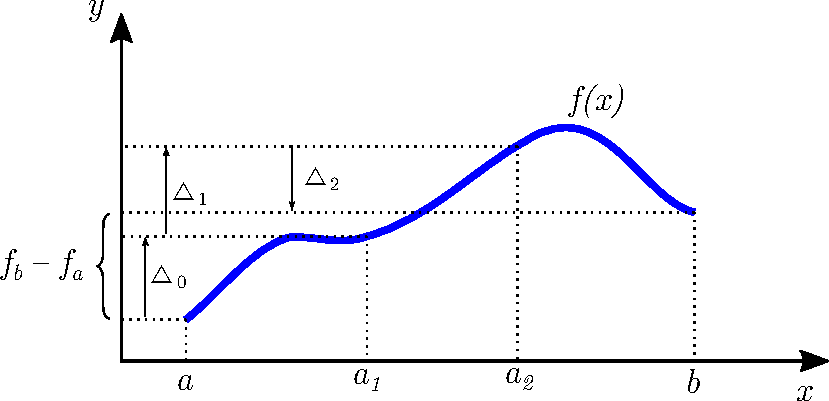
\includegraphics[width=0.6\linewidth]{div1d.pdf}
\caption{Формула Гаусса-Остроградского в одномерном случае}
\label{fig:div1d}
\end{figure}
Разобъем область на $N=3$ равномерных подобласти длины $h$. Тогда
расписывая интеграл как сумму, а производную через конечную разность, получим
$$
\arint{\dfr{f}{x}}{E}{x} \approx \sum_{i=0}^{2} h \left(\dfr{f}{x}\right)_{i+\tfrac12}
\approx\sum_{i=0}^{2}(f_{i+1} - f_{i})
= \triangle_0 + \triangle_1 + \triangle_2 = f_b - f_a.
$$
Очевидно что, при устремлении $N\to\infty$ правая часть предыдущего выражения не изменится.
То есть, сумма всех изменений функции в области есть изменение функции по её границам:
$$
\int\limits_{a}^{b}\dfr{f}{x}\,dx = f(b) - f(a).
$$
А формула \cref{eq:partint_div} -- есть многомерное обобщение этого выражения.

\subsubsection{Интегрирование по частям}

Подставив в \cref{eq:partint_div} $\vec v = f\vec u$, где $f$ -- некоторая скалярная функция, и 
расписав дивергенцию в виде
$$\nabla\cdot(f\vec u) = f\nabla\vec u + \vec u \cdot \nabla f$$
получим формулу интегрирования по частям
\begin{equation}
\label{eq:partint}
\arint{\vec u \cdot \nabla f}{E}{\vec x} = \arint{f u_n}{\Gamma}{s} - \arint{f\nabla\cdot \vec u}{E}{\vec x}
\end{equation}
Распишем некоторые частные случаи для формулы \cref{eq:partint}.
Для $\vec u = (n_x, 0, 0)$ получим
\begin{equation}
\label{eq:partint_ugrad_}
\arint{\dfr{f}{x}}{E}{\vec x} = \arint{f \cos(\vecangle{n}{x})}{\Gamma}{s}
\end{equation}
При $\vec u = \nabla g$
\begin{equation}
\label{eq:partint_laplace_fg}
\arint{f\left(\nabla^2 g \right)}{E}{\vec x} = \arint{f\dfr{g}{n}}{\Gamma}{s} - \arint{\nabla f \cdot \nabla g}{E}{\vec x}
\end{equation}
При $f=1$ и $\vec u = \nabla g$
\begin{equation}
\label{eq:partint_laplace}
\arint{\nabla^2 g}{E}{\vec x} = \arint{\dfr{g}{n}}{\Gamma}{s}
\end{equation}

\subsubsection{Численное интегрирование в заданной области}
Квадратурная формула
\begin{equation}
\label{eq:quadrature_formula}
\arint{f(\vec x)}{E}{\vec x} = \sum_{i=0}^{N-1} w_i f(\vec x_i)
\end{equation}
Она определяется заданием узлов интегрирования $\vec x_i$ 
и соответствующих весов $w_i$.

\subsection{Интерполяционные полиномы}

\subsubsection{Многочлен Лагранжа}

\subsubsubsection{Узловые базисные функции}

Рассмотрим функцию $f(\xi)$, заданную в области $D$.
Внутри этой области зададим $N$ узловых
точек $\xi_i, i=\overline{0,N-1}$.
Приближение функции $f$ будем искать в виде
\begin{equation}
\label{eq:nodal_basis}
f(\xi) \approx \sum_{i=0}^{N-1} f_i \phi_i(\xi),
\end{equation}
где  $f_i = f(\xi_i)$, $\phi_i$ -- узловая базисная функция.
Потребуем, чтобы это выражение выполнялось точно для всех
заданных узлов интерполяции $\xi = \xi_i$. Тогда, исходя из определения \cref{eq:nodal_basis}, запишем условие 
на узловую базисную функцию
\begin{equation}
\label{eq:nodal_bases_conditions}
\phi_i(\xi_j) = 
\begin{cases}
1, &\quad i = j, \\
0, &\quad i \neq j.
\end{cases}
\end{equation}
Дополнительно потребуем, чтобы формула \cref{eq:nodal_basis} была
точной для постоянных функций
$$
f(\xi)=\const \hence f_i = \const.
$$
Тогда для любого $\xi$ должно выполняться условие
\begin{equation}
\label{eq:nodal_bases_unitsum}
\sum_{i=0}^{N-1} \phi_i(\xi) = 1, \qquad \xi \in D.
\end{equation}

Задача построения интерполяционной функции состоит
в конкретном определении узловых базисов
$\phi_i(\xi)$ по заданному набору
узловых точек $\xi_i$ и значениям
функции в них $f_i$. Будем искать базисы
в виде многочленов вида
\begin{equation}
\label{eq:nodal_basis_1d_decomp}
\phi_i(\xi) = \sum_{a} A_i^{(a)} \xi^{a} =
A_i^{(0)} + 
A_i^{(1)} \xi + 
A_i^{(2)} \xi^2 +  \ldots, \qquad i = \overline{0, N-1}.
\end{equation}
Определять коэффициенты $A^{(a)}_i$ будем из условий \cref{eq:nodal_bases_conditions},
которое даёт $N$ линейных уравнений относительно неизвестных $A_i^{(a)}$ для каждого $i=\overline{0, N-1}$.
Таким образом, в выражениях \cref{eq:nodal_basis_1d_decomp} должно быть
ровно $N$ слагаемых.
Будем использовать последовательный набор степеней: $a=\overline{0,N-1}$.
Выпишем систему линейных уравнений для $0$-ой базисной функции
\begin{equation*}
\begin{aligned}
& \phi_0(\xi_0) = A_0^{(0)} + A_0^{(1)} \xi_0 + A_0^{(2)} \xi_0^2 + A_0^{(3)} \xi_0^3 + \ldots = 1, \\
& \phi_0(\xi_1) = A_0^{(0)} + A_0^{(1)} \xi_1 + A_0^{(2)} \xi_1^2 + A_0^{(3)} \xi_1^3 + \ldots = 0, \\
& \phi_0(\xi_2) = A_0^{(0)} + A_0^{(1)} \xi_2 + A_0^{(2)} \xi_2^2 + A_0^{(3)} \xi_2^3 + \ldots = 0, \\
& \ldots
\end{aligned}
\end{equation*}
или в матричном виде
\begin{equation*}
\left(
\begin{array}{ccccc}
1 & \xi_0 & \xi_0^2 & \xi_0^3 & \ldots \\[5pt]
1 & \xi_1 & \xi_1^2 & \xi_1^3 & \ldots \\[5pt]
1 & \xi_2 & \xi_2^2 & \xi_2^3 & \ldots \\[5pt]
1 & \xi_3 & \xi_3^2 & \xi_3^3 & \ldots \\[5pt]
\ldots &&&&
\end{array}
\right)
\left(
\begin{array}{c}
A_0^{(0)} \\[5pt]
A_0^{(1)} \\[5pt]
A_0^{(2)} \\[5pt]
A_0^{(3)} \\[5pt]
\vdots
\end{array}
\right)
=
\left(
\begin{array}{c}
1 \\[5pt]
0 \\[5pt]
0 \\[5pt]
0 \\[5pt]
\vdots
\end{array}
\right)
\end{equation*}
Записывая аналогичные выражения для остальных базисных функций, получим систему матричных уравнений
вида $C A = E$:
\begin{equation*}
\left(
\begin{array}{ccccc}
1 & \xi_0 & \xi_0^2 & \xi_0^3 & \ldots \\[5pt]
1 & \xi_1 & \xi_1^2 & \xi_1^3 & \ldots \\[5pt]
1 & \xi_2 & \xi_2^2 & \xi_2^3 & \ldots \\[5pt]
1 & \xi_3 & \xi_3^2 & \xi_3^3 & \ldots \\[5pt]
\ldots &&&&
\end{array}
\right)
\left(
\begin{array}{ccccc}
A_0^{(0)} & A_1^{(0)} & A_2^{(0)} & A_3^{(0)} & \ldots\\[5pt]
A_0^{(1)} & A_1^{(1)} & A_2^{(1)} & A_3^{(1)} &       \\[5pt]
A_0^{(2)} & A_1^{(2)} & A_2^{(2)} & A_3^{(2)} &       \\[5pt]
A_0^{(3)} & A_1^{(3)} & A_2^{(3)} & A_3^{(3)} &       \\[5pt]
\vdots
\end{array}
\right)
=
\left(
\begin{array}{ccccc}
1 & 0 & 0 & 0 & \ldots \\[5pt]
0 & 1 & 0 & 0 &        \\[5pt]
0 & 0 & 1 & 0 &        \\[5pt]
0 & 0 & 0 & 1 &        \\[5pt]
\vdots
\end{array}
\right)
\end{equation*}
Отсюда матрица неизвестных коэффициентов $A$ определится как
\begin{equation}
\label{eq:nodal_basic_amat}
A = C^{-1} = 
\left(
\begin{array}{ccccc}
1 & \xi_0 & \xi_0^2 & \xi_0^3 & \ldots \\[5pt]
1 & \xi_1 & \xi_1^2 & \xi_1^3 & \ldots \\[5pt]
1 & \xi_2 & \xi_2^2 & \xi_2^3 & \ldots \\[5pt]
1 & \xi_3 & \xi_3^2 & \xi_3^3 & \ldots \\[5pt]
\ldots &&&&
\end{array}
\right) ^{-1}.
\end{equation}

Подставляя полином \cref{eq:nodal_basis_1d_decomp} в условие согласованности \cref{eq:nodal_bases_unitsum},
получим требование
\begin{equation*}
\sum_{i=0}^{N-1} A_i^{(a)} = 
\begin{cases}
1, \quad a=0, \\
0, \quad a=\overline{1,N-1}.
\end{cases}
\end{equation*} 
То есть сумма всех свободных членов в интерполяционных полиномах должна
быть равна единице, а сумма коэффициентов при остальных степенях -- нулю.
Можно показать, что это свойство выполняется для любой матрицы $A=C^{-1}$,
в случае, если первый столбец матрицы $C$ состоит из единиц.
То есть условие согласованности требует наличие свободного члена
с интерполяционном полиноме.


\subsubsubsection{Интерполяция в параметрическом отрезке}
\label{sec:segment_bases}
Будем рассматривать область интерполяции $D=[-1, 1]$.
В качестве первых двух узлов интерполяции возьмем границы области:
$\xi_0 = -1$, $\xi_1 = 1$.
\paragraph{Линейный базис}
Будем искать интерполяционный базис в виде
$$
\phi_i(\xi) = A_i^{(0)} + A_i^{(1)} \xi.
$$
на основе двух условий:
$$
\phi_i(-1) = A_i^{(0)} - A_i^{(1)} = \delta_{0i}, \quad \phi_i(1) = A_i^{(0)} + A_i^{(1)}\delta_{1i}.
$$
Составим матрицу $C$, записав эти условия в матричном виде
$$
C =
\left(
\begin{array}{l|rr}
      & A^{(0)} & A^{(1)}\\
\hline
\phi(-1) & 1 & -1 \\[5pt]
\phi(1) & 1 &  1 \\[5pt]
\end{array}
\right)
$$
и, согласно \cref{eq:nodal_basic_amat}, найдём матрицу коэффициентов
$$
A =
\left(
\begin{array}{cc}
A_0^{(0)} & A_1^{(0)} \\[5pt]
A_0^{(1)} & A_1^{(1)} \\[5pt]
\end{array}
\right) = C^{-1} =
\left(
\begin{array}{l|rr}
     & \phi_0   & \phi_1  \\
\hline
1    & \frac12  & \frac12 \\[5pt]
\xi  & -\frac12 & \frac12 \\[5pt]
\end{array}
\right).
$$
Отсюда узловые базисные функции примут вид (\figref{fig:basis1d_linear})
\begin{equation}
\label{eq:segment_linear_basis}
\begin{aligned}
&\phi_0(\xi) = \frac{1 - \xi}{2}, \\
&\phi_1(\xi) = \frac{1 + \xi}{2}.
\end{aligned}
\end{equation}
Окончательно интерполяционная функция из определения \cref{eq:nodal_basis}
примет вид
$$
f(\xi) \approx \frac{1 - \xi}{2} f(-1) + \frac{1 + \xi}{2} f(1).
$$
\begin{figure}[h!]
\centering
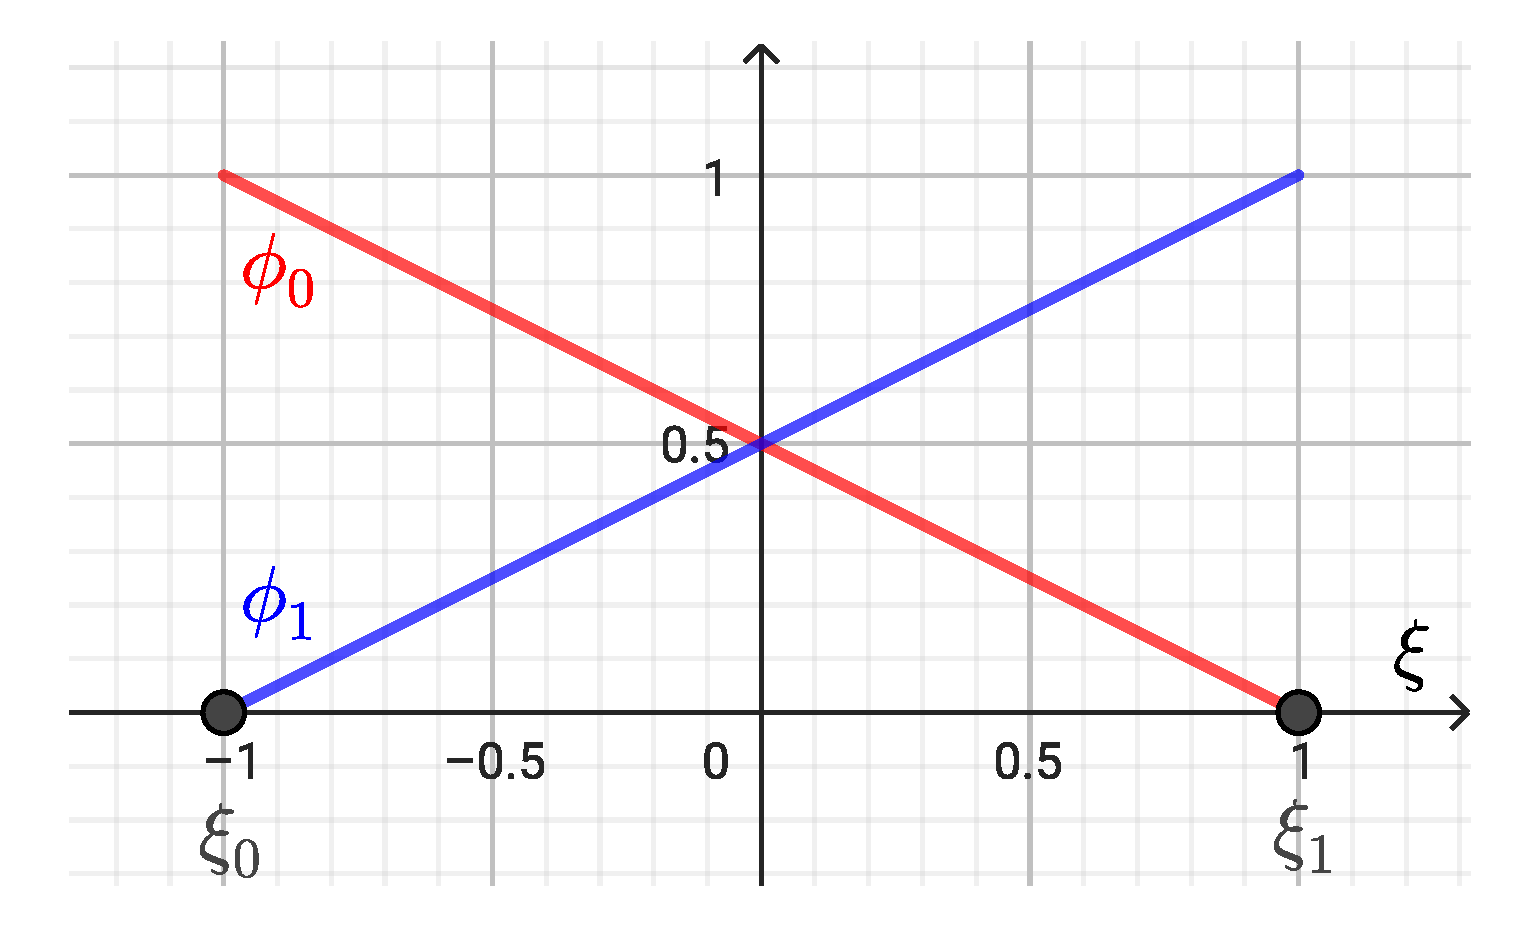
\includegraphics[width=0.4\linewidth]{basis1d_linear.pdf}
\caption{Линейный базис в параметрическом отрезке}
\label{fig:basis1d_linear}
\end{figure}

\paragraph{Квадратичный базис}
Будем искать интерполяционный базис в виде
$$
\phi_i(\xi) = A_i^{(0)} + A_i^{(1)} \xi + A_i^{(2)} \xi^2.
$$
По сравнению с линейным случаем, в форму базиса добавился ещё один неизвестый коэффициент $A_i^{(2)}$,
поэтому в набор условий \cref{eq:nodal_bases_conditions} требуется ещё одно уравнение (ещё одна узловая точка).
Поместим её в центр параметрического сегмента $\xi_2 = 0$. Далее будем действовать по
аналогии с линейным случаем:
$$
C = \left(
\begin{array}{l|rrr}
         &  A^{(0)} & A^{(1)}   & A^{(2)} \\ 
\hline
\phi(-1) & 1 & -1 & 1\\[5pt]
\phi(1)  & 1 &  1 & 1\\[5pt]
\phi(0)  & 1 &  0 & 0
\end{array}
\right)
\hence
A = C^{-1} = \left(
\begin{array}{l|rrr}
       & \phi_0   & \phi_1   & \phi_2 \\
\hline
 1     & 0        &  0       &  1     \\[5pt]
 \xi   & -\frac12 &  \frac12 &  0     \\[5pt]
 \xi^2 &  \frac12 &  \frac12 & -1     \\[5pt]
\end{array}
\right).
$$
Узловые базисные функции для квадратичной интерполяции примут вид (\figref{fig:basis1d_quadratic})
\begin{equation}
\label{eq:segment_quadratic_basis}
\begin{aligned}
&\phi_0(\xi) = \frac{\xi^2 - \xi}{2}, \\
&\phi_1(\xi) = \frac{\xi^2 + \xi}{2}, \\
&\phi_2(\xi) = 1 - \xi^2.
\end{aligned}
\end{equation}

\begin{figure}[h!]
\centering
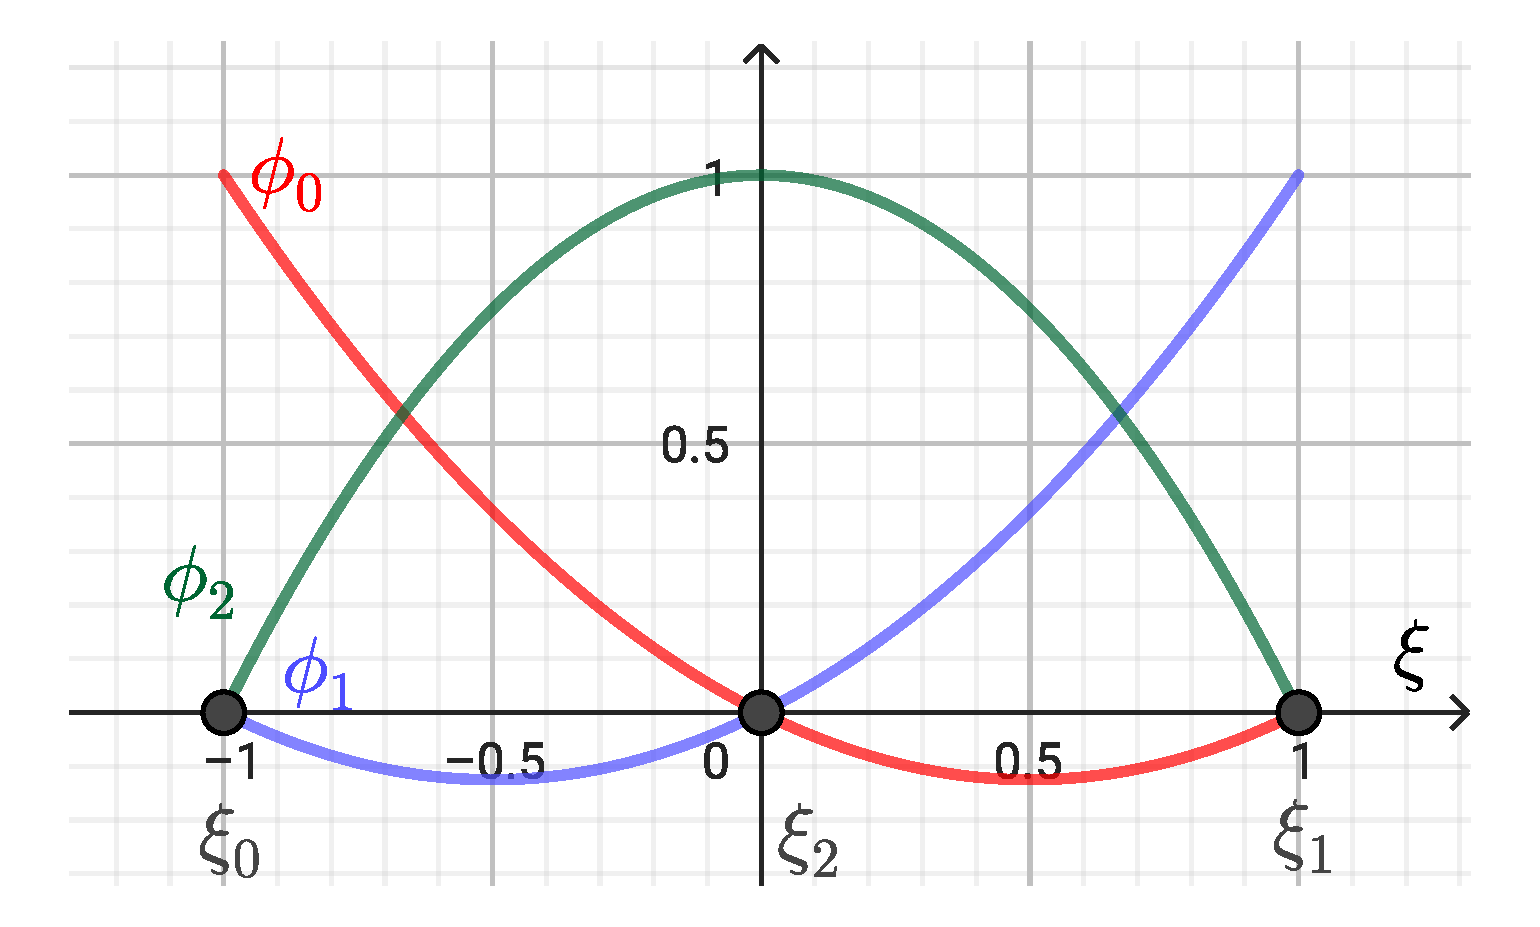
\includegraphics[width=0.4\linewidth]{basis1d_quadratic.pdf}
\caption{Квадратичный базис в параметрическом отрезке}
\label{fig:basis1d_quadratic}
\end{figure}

\paragraph{Кубический базис}
Интерполяционный базис будет иметь вид
$$
\phi_i(\xi) = A_i^{(0)} + A_i^{(1)} \xi + A_i^{(2)} \xi^2 + A_i^{(3)} \xi^3.
$$
Для нахождения четырёх коэффициентов нам понадобится четыре узла интерполяции.
Две из них -- это границы параметрического отрезка. Остальные две разместим
так, чтобы разбить отрезок на равные интервалы:
$\xi_2 = -\tfrac13$, $\xi_3 = \tfrac13$.
Далее вычислим матрицу коэффициентов:
$$
C =
\left(
\begin{array}{l|rrrr}
                &  A^{(0)}  &  A^{(1)}      & A^{(2)}     & A^{(3)}         \\
\hline
\phi(-1)        &  1  & -1        & 1         &  -1           \\[5pt]
\phi( 1)        &  1  & 1         & 1         &   1           \\[5pt]
\phi(-\tfrac13) &  1  & -\tfrac13 & \tfrac19  &  -\tfrac1{27} \\[5pt]
\phi(\tfrac13)  &  1  &  \tfrac13 & \tfrac19  &   \tfrac1{27}
\end{array}
\right)
\hence
A = C^{-1} =
\frac{1}{16}
\left(
\begin{array}{l|rrrr}
      & \phi_0 & \phi_1 & \phi_2 & \phi_3 \\
\hline
1     & -1     & -1     &   9    &  9     \\[5pt]
\xi   &  1     & -1     & -27    &  27    \\[5pt]
\xi^2 &  9     &  9     & -9     & -9     \\[5pt]
\xi^3 & -9     &  9     &  27    & -27   
\end{array}
\right)
$$
Узловые базисные функции для квадратичной интерполяции примут вид (\figref{fig:basis1d_cubic})
\begin{equation}
\label{eq:segment_cubic_basis}
\begin{aligned}
&\phi_0(\xi) = \frac{1}{16}\left(-1 + \xi + 9 \xi^2 -9 \xi^3\right), \\
&\phi_1(\xi) = \frac{1}{16}\left(-1 - \xi + 9 \xi^2 +9 \xi^3\right), \\
&\phi_2(\xi) = \frac{1}{16}\left(9 -27 \xi - 9\xi^2 + 27 \xi^3\right), \\
&\phi_3(\xi) = \frac{1}{16}\left(9 +27 \xi - 9\xi^2 - 27 \xi^3\right), \\
\end{aligned}
\end{equation}

\begin{figure}[h!]
\centering
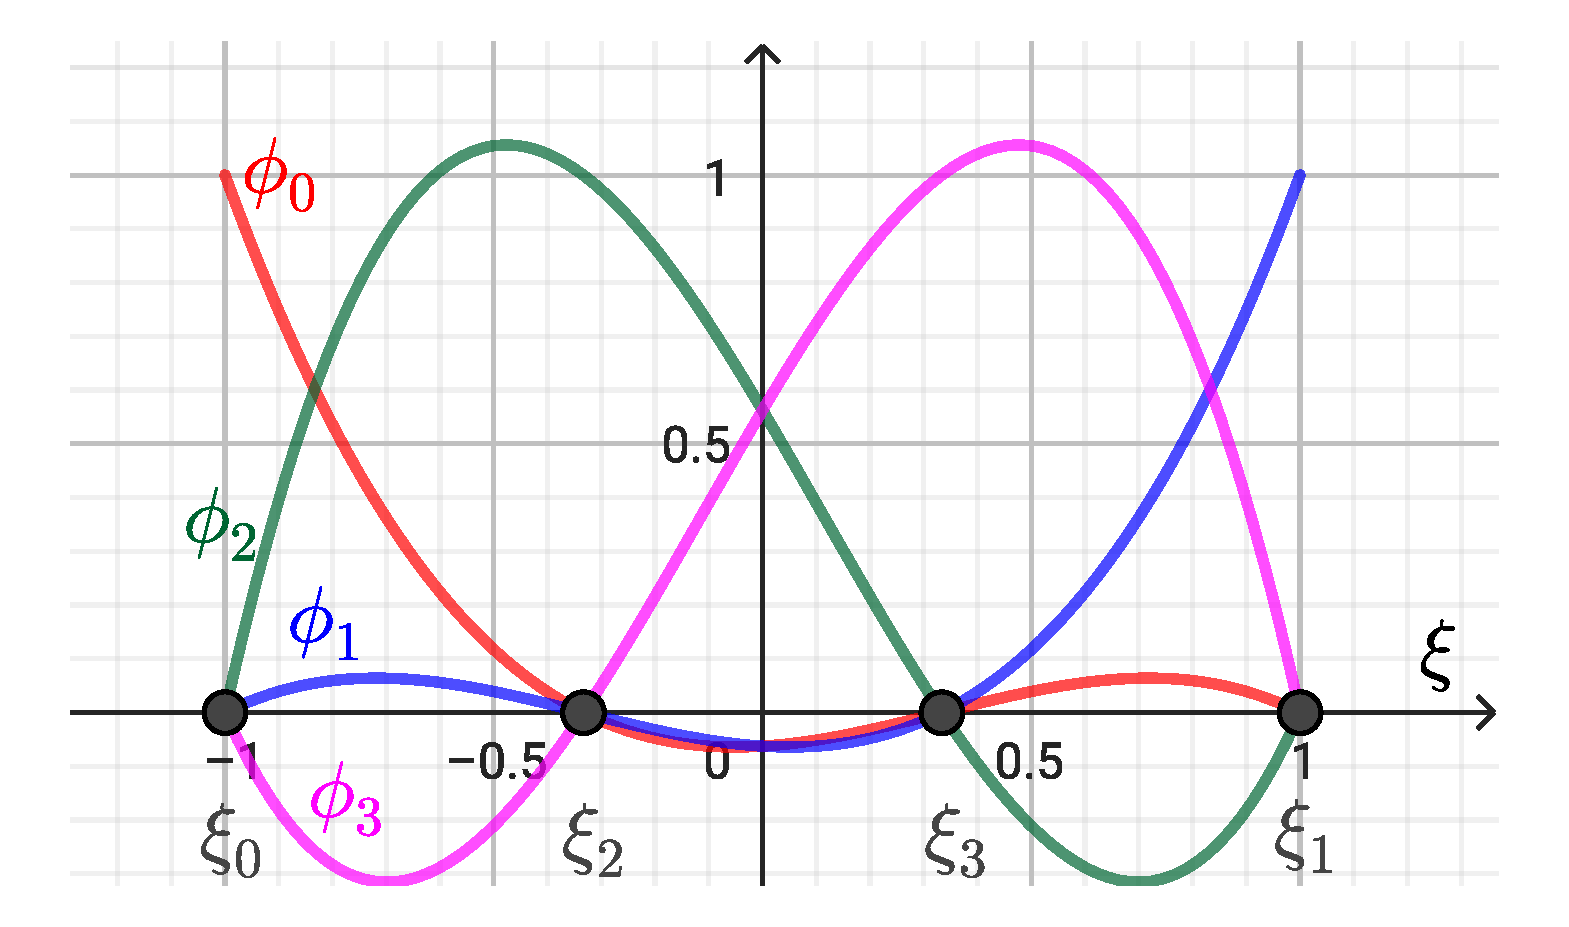
\includegraphics[width=0.4\linewidth]{basis1d_cubic.pdf}
\caption{Кубический базис в параметрическом отрезке}
\label{fig:basis1d_cubic}
\end{figure}

На \figref{fig:basis1d_compare} представлено сравнение результатов
аппроксимации функции $f(x) = -x + \sin(2 x + 1)$ линейным, квадратичным и кубическим базисом.
Видно, что все интерполяционные приближения точно попадают в функцию в своих
узлах интерполяции, а между узлами происходит аппроксимация полиномом соответствующей степени.

\begin{figure}[h!]
\centering
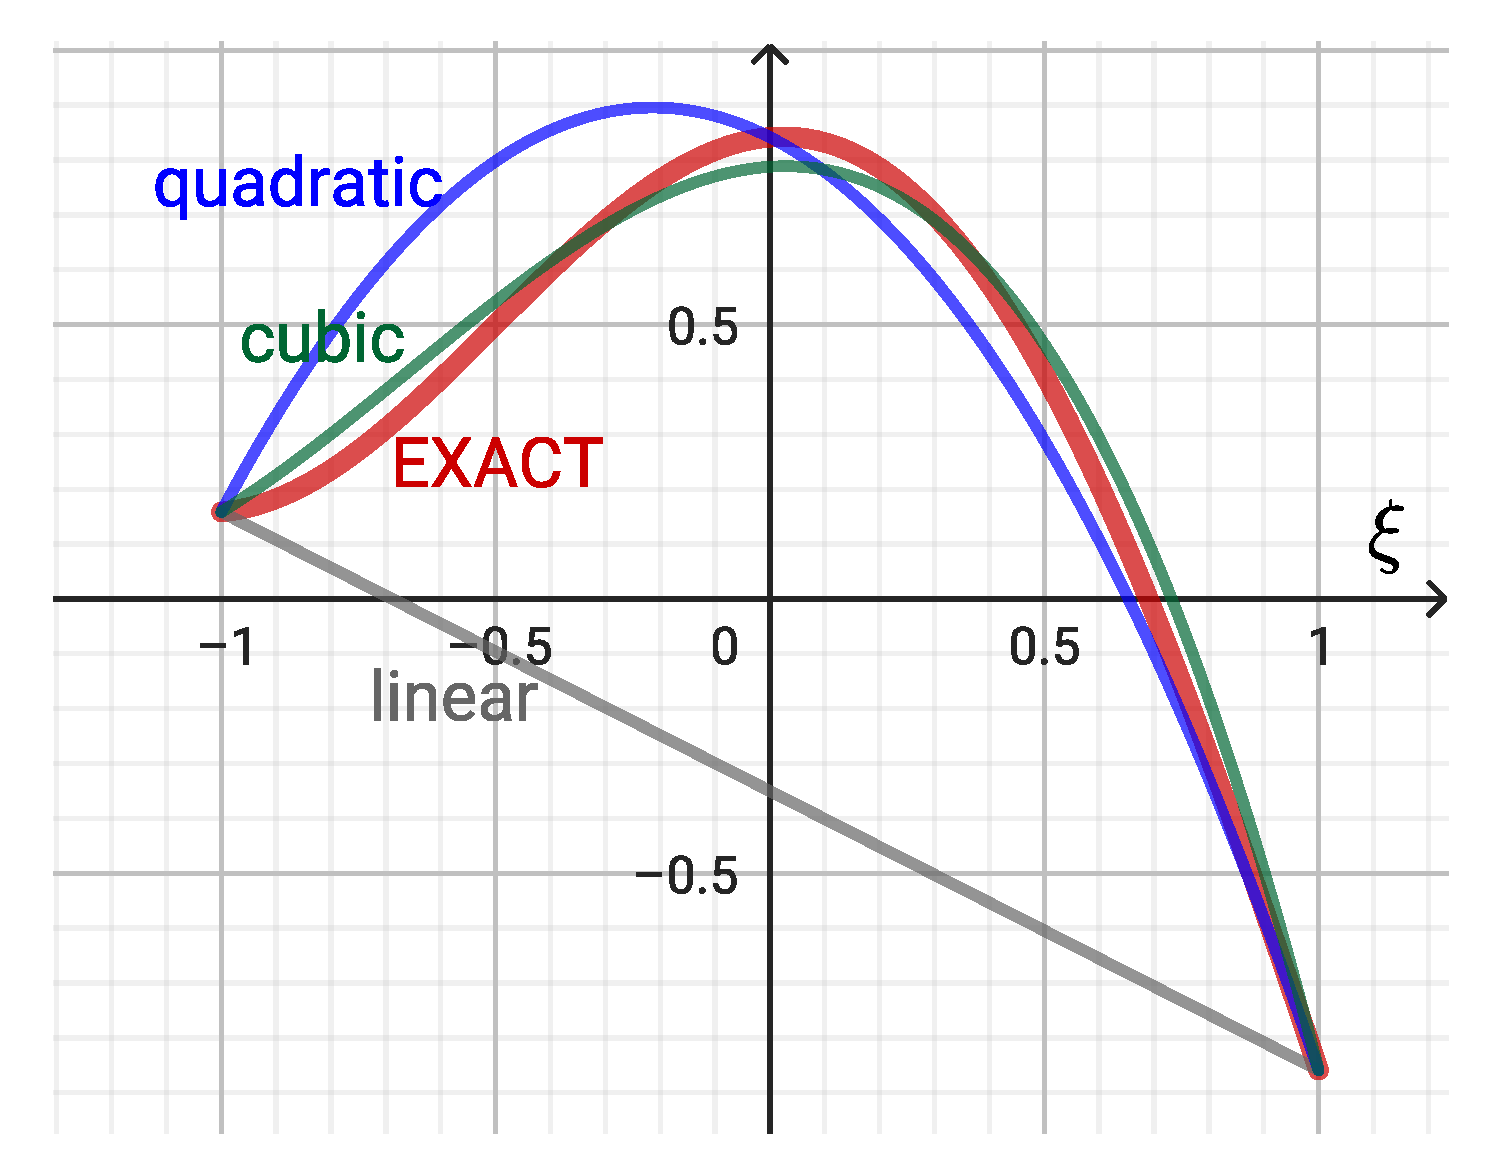
\includegraphics[width=0.4\linewidth]{basis1d_compare.pdf}
\caption{Результат интерполяции}
\label{fig:basis1d_compare}
\end{figure}

\subsubsubsection{Интерполяция в параметрическом треугольнике}
\label{sec:triangle_bases}
Теперь рассмотрим двумерное обобщение формулы
\begin{figure}[h!]
\centering
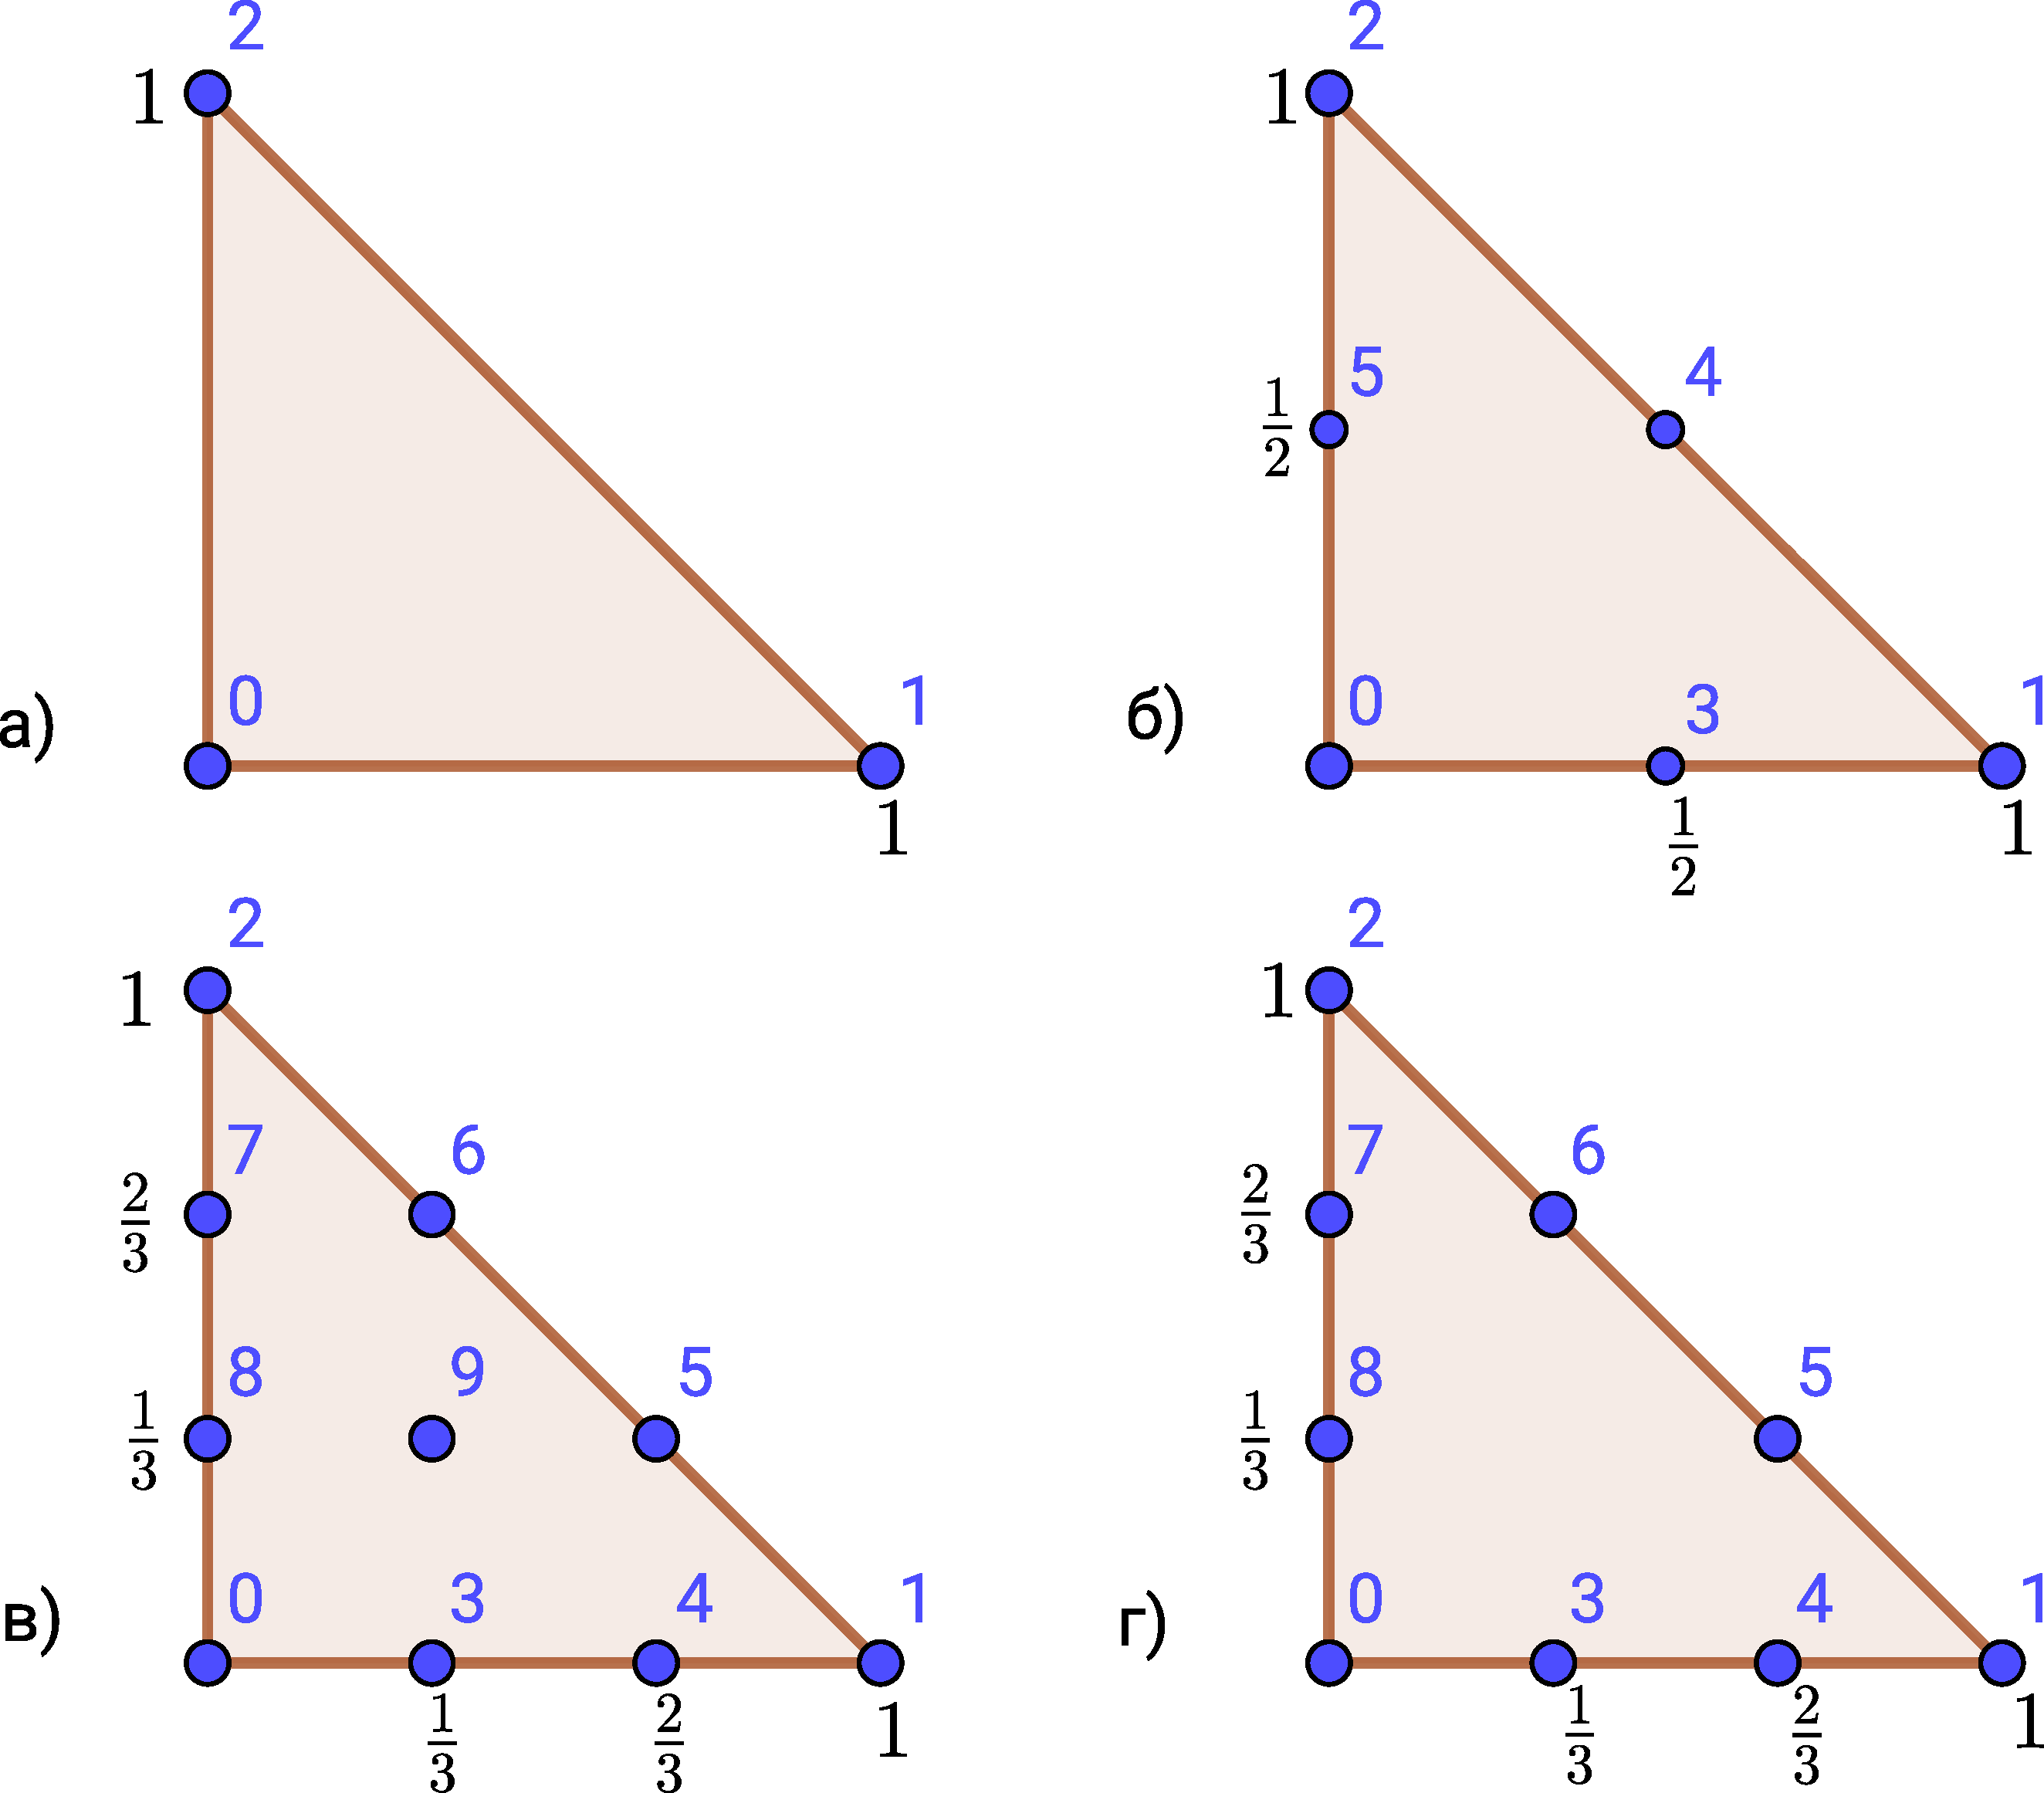
\includegraphics[width=0.5\linewidth]{triangle_basis_points.pdf}
\caption{Расположение узловых точек в параметрическом треугольнике. а) линейный базис, б) квадратичный базис, в) кубический базис, г) неполный кубический базис}
\label{fig:triangle_basis_points}
\end{figure}
\paragraph{Линейный базис}

\begin{equation*}
\phi_i(\xi, \eta) = A_i^{(00)} + A_i^{(10)} \xi + A_i^{(01)} \eta.
\end{equation*}
\begin{equation*}
C = \left(
\begin{array}{l|ccc}
                  & A^{(00)}   & A^{(10)} & A^{(01)} \\
\hline
\phi(0, 0) & 1   & 0   & 0    \\[5pt]
\phi(1, 0) & 1   & 1   & 0    \\[5pt]
\phi(0, 1) & 1   & 0   & 1
\end{array}
\right)
\hence
A = C^{-1} = 
\left(
\begin{array}{l|rrr}
     & \phi_0 & \phi_1 & \phi_2 \\
\hline
1    & 1      & 0      & 0      \\[5pt]
\xi  &-1      & 1      & 0      \\[5pt]
\eta &-1      & 0      & 1
\end{array}
\right)
\end{equation*}

\begin{equation}
\label{eq:triangle_linear_basis}
\begin{aligned}
&\phi_0(\xi, \eta) = 1 - \xi - \eta, \\
&\phi_1(\xi, \eta) = \xi, \\
&\phi_2(\xi, \eta) = \eta, \\
\end{aligned}
\end{equation}

\begin{figure}[h!]
\centering
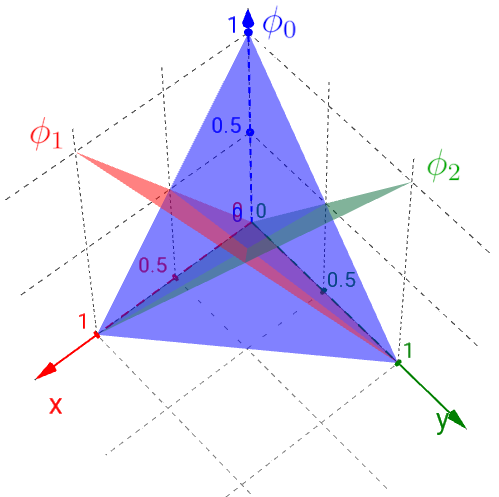
\includegraphics[width=0.4\linewidth]{basis2d_linear.png}
\caption{Линейный базис в параметрическом треугольнике}
\label{fig:basis2d_linear}
\end{figure}


\paragraph{Квадратичный базис}
\begin{equation*}
\phi_i(\xi, \eta) = A_i^{(00)} + A_i^{(10)} \xi + A_i^{(01)} \eta + A_i^{(11)} \xi \eta + A_i^{(20)} \xi^2 + A_i^{(02)} \eta^2.
\end{equation*}

\begin{equation*}
C =
\left(
\begin{array}{l|cccccc}
                     & A^{(00)} & A^{(10)}      & A^{(01)}  & A^{(11)}  & A^{(20)}    & A^{(02)}   \\[5pt]
\hline
\phi(0, 0)               & 1 &  0       &  0          &   0      &    0     &   0      \\[5pt]
\phi(1, 0)               & 1 &  1       &  0          &   0      &    1     &   0      \\[5pt]
\phi(0, 1)               & 1 &  0       &  1          &   0      &    0     &   1      \\[5pt]
\phi(\tfrac12, 0)        & 1 & \tfrac12 &  0          &   0      & \tfrac14 &   0      \\[5pt]
\phi(\tfrac12, \tfrac12) & 1 & \tfrac12 &  \tfrac12   & \tfrac14 & \tfrac14 & \tfrac14 \\[5pt]
\phi(0, \tfrac12)        & 1 &  0       &  \tfrac12   &   0      &    0     & \tfrac14 
\end{array}
\right)
\hence
A = \left(
\begin{array}{l|rrrrrr}
        & \phi_0 & \phi_1 & \phi_2 & \phi_3 & \phi_4 & \phi_5 \\[5pt]
\hline
1       & 1  &  0 & 0 & 0 & 0 & 0\\[5pt]
\xi     & -3 & -1 & 0 & 4 & 0 & 0\\[5pt]
\eta    & -3 & 0 & -1 & 0 & 0 & 4\\[5pt]
\xi\eta & 4 & 0 & 0 & -4 & 4 & -4\\[5pt]
\xi^2   & 2 & 2 & 0 & -4 & 0 & 0 \\[5pt]
\eta^2  & 2 & 0 & 2 & 0 & 0 & -4
\end{array}
\right)
\end{equation*}

\begin{figure}[h!]
\centering
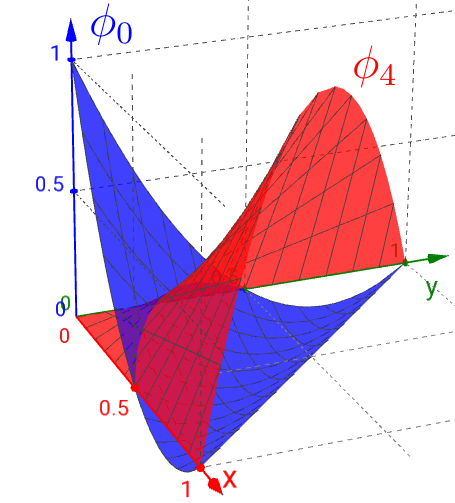
\includegraphics[width=0.3\linewidth]{basis2d_quadratic.png}
\caption{Квадратичные функции $\phi_0$, $\phi_4$ в параметрическом треугольнике}
\label{fig:basis2d_quadratic}
\end{figure}

\paragraph{Кубический базис}
TODO

\paragraph{Неполный кубический базис}
TODO

\subsubsubsection{Интерполяция в параметрическом квадрате}
\begin{figure}[h!]
\centering
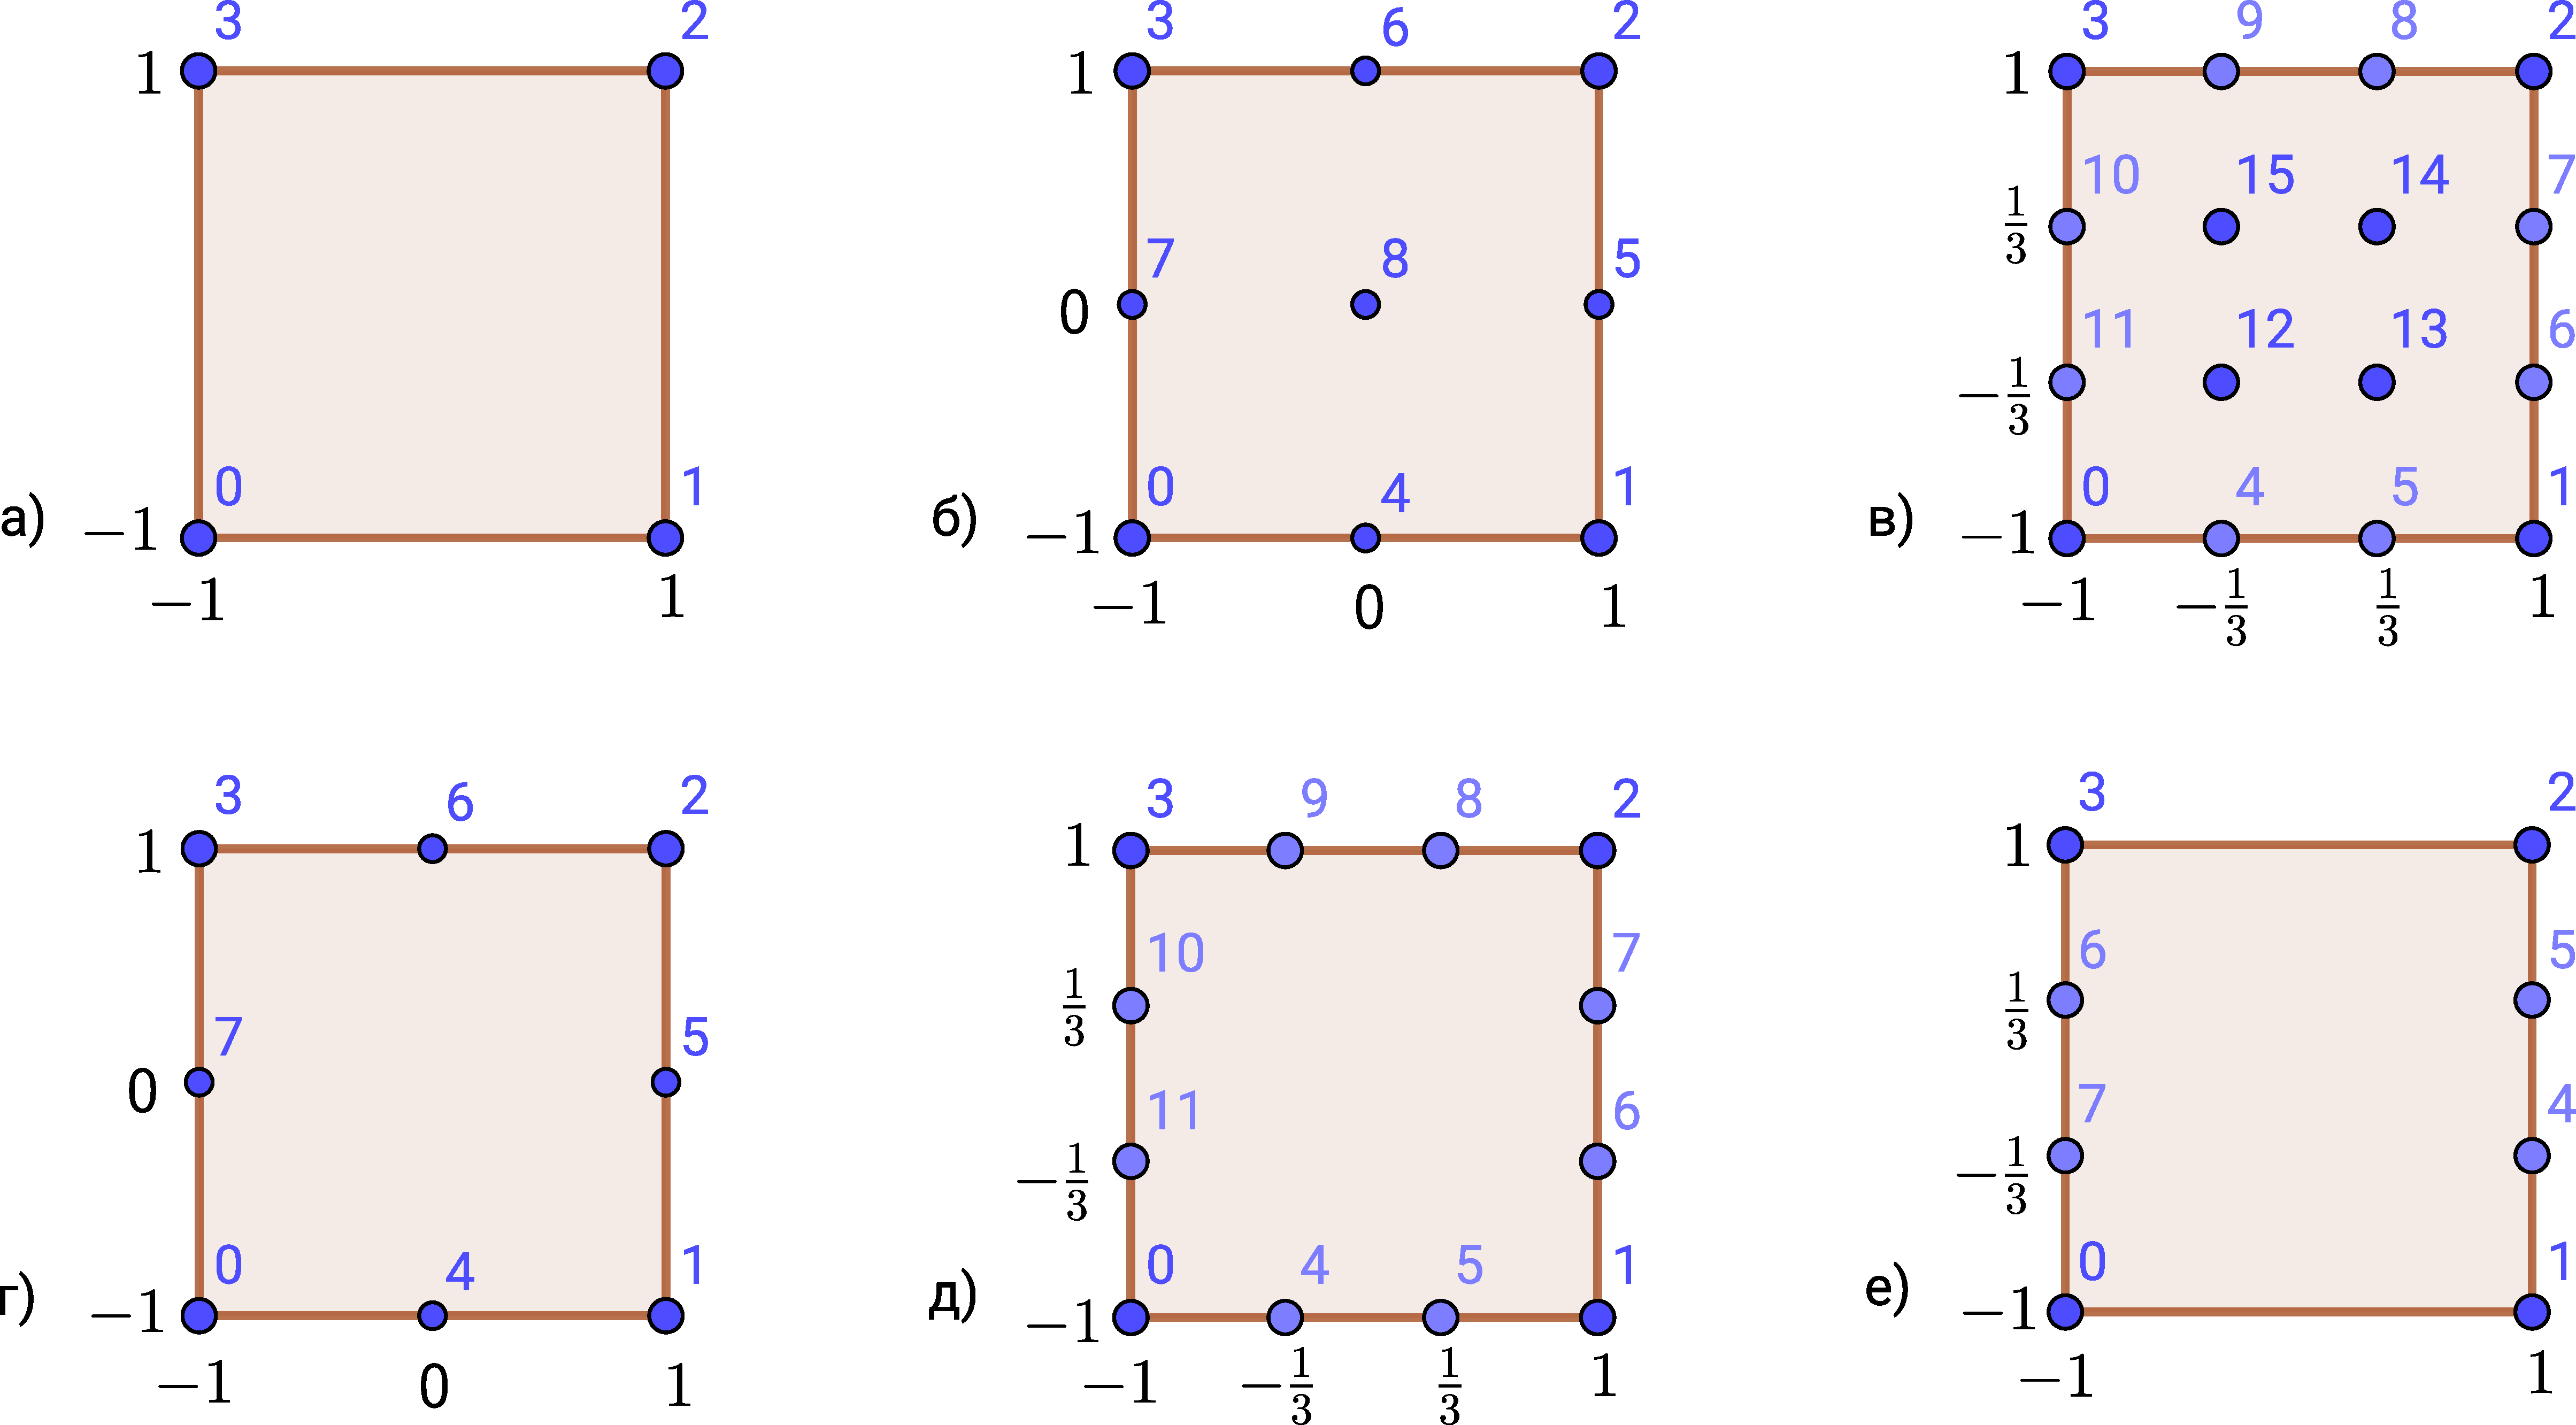
\includegraphics[width=0.7\linewidth]{quadrangle_basis_points.pdf}
\caption{Расположение узловых точек в параметрическом квадратре}
\label{fig:quadrangle_basis_points}
\end{figure}

\paragraph{Билинейный базис}
\begin{equation*}
\phi_i = A^{00}_i + A^{10}_i \xi + A^{01}_i \eta + A^{11}_i \xi\eta.
\end{equation*}

\begin{equation*}
C = \left(
\begin{array}{l|rrrr}
                      & A^{(00)} & A^{(10)} & A^{(01)} & A^{(11)} \\
\hline
\phi(-1, -1) & 1 & -1  & -1   &  1      \\[5pt] 
\phi( 1, -1) & 1 &  1  & -1   & -1      \\[5pt]
\phi( 1,  1) & 1 &  1  &  1   &  1      \\[5pt]
\phi(-1,  1) & 1 & -1  &  1   & -1      \\[5pt]
\end{array}
\right)
\hence
A = C^{-1} = \frac14\left(
\begin{array}{l|rrrr}
        & \phi_0 & \phi_1 & \phi_2 & \phi_3\\
\hline
1       & 1 & 1 & 1 & 1\\[5pt]
\xi     & -1 & 1 & 1 & -1\\[5pt]
\eta    & -1 & -1 & 1 & 1\\[5pt]
\xi\eta & 1 & -1 & 1 & -1
\end{array}
\right)
\end{equation*}

\begin{equation}
\label{eq:quadrangle_bilinear_basis}
\begin{aligned}
&\phi_0(\xi, \eta) = \frac{1-\xi-\eta+\xi\eta}{4}\\[10pt]
&\phi_1(\xi, \eta) = \frac{1+\xi-\eta-\xi\eta}{4}\\[10pt]
&\phi_2(\xi, \eta) = \frac{1+\xi+\eta+\xi\eta}{4}\\[10pt]
&\phi_3(\xi, \eta) = \frac{1-\xi+\eta-\xi\eta}{4}
\end{aligned}
\end{equation}

\begin{figure}[h!]
\centering
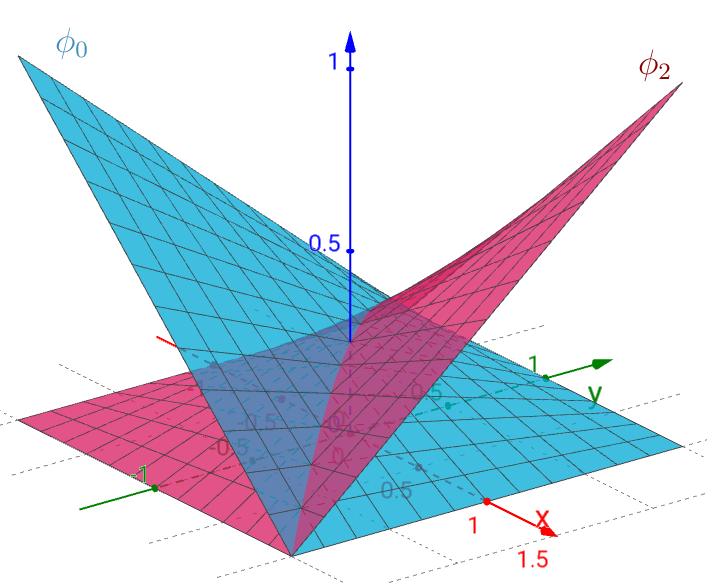
\includegraphics[width=0.4\linewidth]{basis2d_bilinear.png}
\caption{Билинейные функции $\phi_0$, $\phi_2$ в параметрическом квадрате}
\label{fig:basis2d_bilinear}
\end{figure}

\paragraph{Определение двумерных базисов через комбинацию одномерных}
Обратим внимание, что в искомые билинейные базисные функции линейны
в каждом из направлений $\xi, \eta$, если брать их по отдельности.
Значит можно представить эти функции как комбинацию одномерных
линейных базисов \cref{eq:segment_linear_basis} в каждом из направлений.
Узлы двумерного параметрического квадрата можно
выразить через узлы линейного базиса в параметрическом одномерном сегменте,
рассмотренном в п.~\ref{sec:segment_bases}:
$$
\vec \xi_0 = \left(\xi^{1D}_0, \xi^{1D}_0\right), \quad
\vec \xi_1 = \left(\xi^{1D}_1, \xi^{1D}_0\right), \quad
\vec \xi_2 = \left(\xi^{1D}_1, \xi^{1D}_1\right), \quad
\vec \xi_3 = \left(\xi^{1D}_0, \xi^{1D}_1\right).
$$
Значит и соответствующие базисные функции можно выразить
через линейный одномерный базис $\phi^{1D}$ из соотношений \cref{eq:segment_linear_basis}:
\begin{equation*}
\begin{aligned}
\phi_0(\xi, \eta) = \phi_0^{1D}(\xi)\phi^{1D}_0(\eta) = \frac{1-\xi}{2}\frac{1-\eta}{2},\\[5pt]
\phi_1(\xi, \eta) = \phi_1^{1D}(\xi)\phi^{1D}_0(\eta) = \frac{1+\xi}{2}\frac{1-\eta}{2},\\[5pt]
\phi_2(\xi, \eta) = \phi_1^{1D}(\xi)\phi^{1D}_1(\eta) = \frac{1+\xi}{2}\frac{1+\eta}{2},\\[5pt]
\phi_3(\xi, \eta) = \phi_0^{1D}(\xi)\phi^{1D}_1(\eta) = \frac{1-\xi}{2}\frac{1+\eta}{2}.
\end{aligned}
\end{equation*}
Раскрыв скобки можно убедится, что мы получили тот же билинейный базис, что и ранее \cref{eq:quadrangle_bilinear_basis}.

\paragraph{Биквадратичный базис}
Применим этот метод для вычисления биквадратичного базиса, определённого в точках на \figref{fig:quadrangle_basis_points}б.
В качестве основе возьмём квадратичный одномерный базис $\phi^{1D}_i$ из \cref{eq:segment_quadratic_basis}.
\begin{equation}
\label{eq:quadrangle_quadratic_basis}
\begin{array}{ll}
  \phi_0(\xi, \eta) = \phi_0^{1D}(\xi)\phi_0^{1D}(\eta) = \dfrac{\xi^2 - \xi}{2}\dfrac{\eta^2 - \eta}{2},
& \phi_1(\xi, \eta) = \phi_1^{1D}(\xi)\phi_0^{1D}(\eta) = \dfrac{\xi^2 + \xi}{2}\dfrac{\eta^2 - \eta}{2}, \\[10pt]
  \phi_2(\xi, \eta) = \phi_1^{1D}(\xi)\phi_1^{1D}(\eta) = \dfrac{\xi^2 + \xi}{2}\dfrac{\eta^2 + \eta}{2},
& \phi_3(\xi, \eta) = \phi_0^{1D}(\xi)\phi_1^{1D}(\eta) = \dfrac{\xi^2 - \xi}{2}\dfrac{\eta^2 + \eta}{2}, \\[10pt]
  \phi_4(\xi, \eta) = \phi_2^{1D}(\xi)\phi_0^{1D}(\eta) = (1-\xi^2)\dfrac{\eta^2 - \eta}{2},
& \phi_5(\xi, \eta) = \phi_1^{1D}(\xi)\phi_2^{1D}(\eta) = \dfrac{\xi^2 + \xi}{2}(1 - \eta^2),            \\[10pt]
  \phi_6(\xi, \eta) = \phi_2^{1D}(\xi)\phi_1^{1D}(\eta) = (1-\xi^2)\dfrac{\eta^2 + \eta}{2},
& \phi_7(\xi, \eta) = \phi_0^{1D}(\xi)\phi_2^{1D}(\eta) = \dfrac{\xi^2 - \xi}{2}(1 - \eta^2),            \\[10pt]
  \phi_8(\xi, \eta) = \phi_2^{1D}(\xi)\phi_2^{1D}(\eta) = (1-\xi^2)(1 - \eta^2).
&
\end{array}
\end{equation}

\paragraph{Бикубический базис}

\paragraph{Неполный биквадратичный базис}

\paragraph{Неполный бикубический базис}

\subsection{Геометрические алгоритмы}
\subsubsection{Линейная интерполяция}
\begin{figure}[h!]
\centering
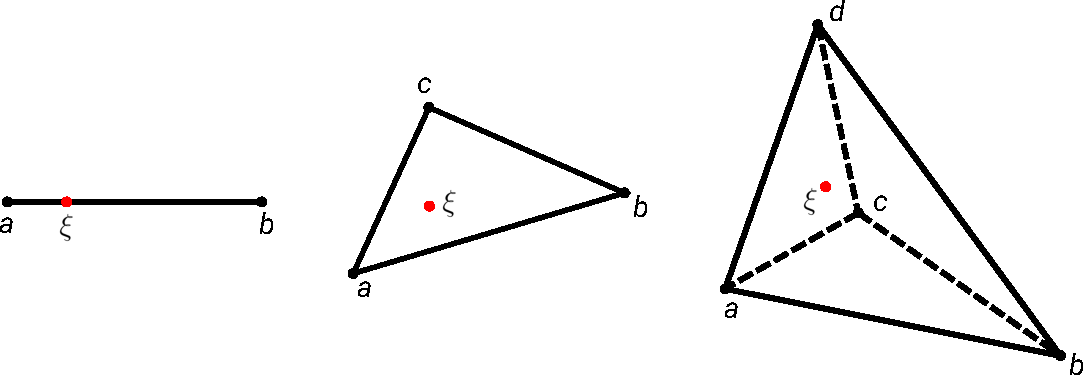
\includegraphics[width=0.8\linewidth]{geom_interp.pdf}
\caption{Порядок нумерации точек одномерного, двумерного и трёхмерного симплекса при линейной интерполяции}
\label{fig:geom_interp}
\end{figure}
Пусть функция $u$ задана в узлах симплекса, имеющего нумерацию согласно рис.~\ref{fig:geom_interp}.
Необходимо найти значение этой функции в точке $\vec \xi$ (эта точка вообще говоря не обязана лежать внутри симлекса).

Интерполяция в одномерном, двумерном и трёхмерном виде запишется как
\begin{align}
\label{eq:simplex_interp_1d}
&u(\xi) =
\frac{
|\triangle_{\xi a}|u(b)+
|\triangle_{b \xi}|u(a)
}
{|\triangle_{ba}|}
\\[10pt]
\label{eq:simplex_interp_2d}
&u(\xi) =
\frac{
|\triangle_{ab\xi}|u(c) +
|\triangle_{bc\xi}|u(a) +
|\triangle_{ca\xi}|u(b)
}
{|\triangle_{abc}|}
\\[10pt]
\label{eq:simplex_interp_3d}
&u(\xi) =
\frac{
|\triangle_{abc\xi}|u(d) +
|\triangle_{cbd\xi}|u(a) +
|\triangle_{cda\xi}|u(b) +
|\triangle_{adb\xi}|u(c)
}
{|\triangle_{abcd}|},
\end{align}
где $|\triangle|$ -- знаковый объём симплекса, вычисляемый как
\begin{align*}
& |\triangle_{ab}| = b - a, \\[10pt]
& |\triangle_{abc}| = \left(\frac{(\vec b - \vec a)\times(\vec c - \vec a)}{2}\right)_z, \\[10pt]
& |\triangle_{abcd}| = \frac{(\vec b - \vec a)\cdot\left((\vec c - \vec a)\times(\vec d - \vec a)\right)}{6}.\\[10pt]
\end{align*}

\subsubsection{Преобразование координат}
\label{sec:coo_transform} 
Рассмотрим преобразование
из двумерной параметрической системы координат $\vec \xi$ 
в физическую систему $\vec x$.
Такое преобразование полностью определяется покоординатными
функциями $\vec x(\vec \xi)$.
Далее получим соотношения, связывающие операции дифференцирования
и интегрирования в физической и параметрической областях.

\subsubsubsection{Матрица Якоби}
Будем рассматривать двумерное преобразование $(\xi, \eta) \to (x, y)$.
Линеаризуем это преобразование (разложим в ряд Фурье до линейного слагаемого)
\begin{align*}
& x(\xi_0 + d\xi, \eta_0 + d\eta) \approx x_0 + \left.\dfr{x}{\xi}\right|_{\xi_0, \eta_0} d\xi
    + \left.\dfr{x}{\eta}\right|_{\xi_0, \eta_0} d\eta, \\
& y(\xi_0 + d\xi, \eta_0 + d\eta) \approx y_0 + \left.\dfr{y}{\xi}\right|_{\xi_0, \eta_0} d\xi
    + \left.\dfr{y}{\eta}\right|_{\xi_0, \eta_0} d\eta,
\end{align*}
где $x_0 = x(\xi_0, \eta_0)$, $y_0 = y(\xi_0, \eta_0)$.
Переписывая это выражение в векторном виде, получим
\begin{equation}
\label{eq:jacobi_linear}
\vec{x}(\vec \xi_0 + \vec{d\xi} ) - \vec{x}_0 = J(\vec \xi_0) \; \vec{d\xi}.
\end{equation}
Матрица $J$ (зависящая от точки приложения в параметрической плоскости) называется матрицей Якоби:
\begin{equation}
\label{eq:jacobi_matrix_2d}
J = \left(
	\begin{array}{cc}
	J_{11} & J_{12}\\[10pt]
	J_{21} & J_{22}\\
	\end{array}
\right)
= \left(
	\begin{array}{cc}
	\ddfr{x}{\xi} & \ddfr{x}{\eta}\\[10pt]
	\ddfr{y}{\xi} & \ddfr{y}{\eta}\\
	\end{array}
\right)
\end{equation}

\paragraph{Якобиан}

\begin{figure}[h!]
\centering
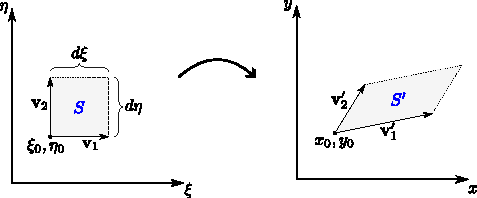
\includegraphics[width=0.6\linewidth]{dxideta.pdf}
\caption{Преобразование элементарного объёма}
\label{fig:dxideta}
\end{figure}

Определитель матрицы Якоби (якобиан), взятый в конкретной точке параметрической плоскости $\vec\xi_0$, показывает,
во сколько раз увеличился элементарный объём около этой точки в результате преобразования.
Действительно, рассмотрим два перпендикулярных элементарных вектора
в параметрической системе координат: $\vec v_1 = (d\xi, 0)$ и $\vec v_2 = (0, d\eta)$
отложенных от точки $\vec\xi_0$ (см.~\figref{fig:dxideta}).
В результате преобразования по формуле \cref{eq:jacobi_linear} 
получим следующие преобразования концевых точек и векторов:
\begin{align*}
& (\xi_0, \eta_0) \to (x_0, y_0), \\
& (\xi_0 + d\xi, \eta_0) \to (x_0 + J_{11} d\xi, y_0 + J_{21} d\xi) \hence \vec v_1 \to \vec v'_1 = (J_{11} d\xi, J_{21} d\xi), \\
& (\xi_0 , \eta_0 + d\eta) \to (x_0 + J_{12} d\eta, y_0 + J_{22} d\eta) \hence \vec v_2 \to \vec v'_2 = (J_{12} d\eta, J_{22} d\eta).
\end{align*}
Элементарный объём равен площади параллелограмма, построенного
на элементарных векторах.
В параметрической плоскости согласно \cref{eq:vec_cross_2d} получим 
$$ |S| = \vec v_1 \times \vec v_2 = d\xi d\eta,$$
и аналогично для физической плоскости:
$$
|S'| = \vec v'_1 \times \vec v'_2 = (J_{11} J_{22} - J_{12} J_{21})d\xi d\eta = |J| d\xi d\eta
$$
Сравнивая два последних соотношения приходим к выводу,
что элементарный объём в результате преобразования увеличился в $|J|$ раз. Тогда можно записать
\begin{equation}
\label{eq:dxdy_dxideta}
dx\,dy = |J|\,d\xi\,d\eta
\end{equation}

\subsubsubsection{Дифференцирование в параметрической плоскости}
Пусть задана некоторая функция $f(x, y)$. Распишем её производную по
параметрическим координатам:
\begin{align*}
&\dfr{f}{\xi} = \dfr{f}{x}\dfr{x}{\xi} + \dfr{f}{y}\dfr{y}{\xi}, \\
&\dfr{f}{\eta} = \dfr{f}{x}\dfr{x}{\eta} + \dfr{f}{y}\dfr{y}{\eta}.
\end{align*}
Вспоминая определение \cref{eq:jacobi_matrix_2d}, запишем
\begin{equation*}
\left(\begin{array}{c}
  \ddfr{f}{\xi} \\[10pt]
  \ddfr{f}{\eta}
  \end{array}
\right) = 
J^T 
\left(
  \begin{array}{c}
  \ddfr{f}{x} \\[10pt]
  \ddfr{f}{y}
  \end{array}
\right) =
\left(
  \begin{array}{cc}
    J_{11} & J_{21} \\[10pt]
    J_{12} & J_{22}
  \end{array}
\right)
\left(
  \begin{array}{c}
  \ddfr{f}{\xi} \\[10pt]
  \ddfr{f}{\eta}
  \end{array}
\right)
\end{equation*}
Обратная зависимость примет вид
\begin{equation*}
\left(\begin{array}{c}
  \ddfr{f}{x} \\[10pt]
  \ddfr{f}{y}
  \end{array}
\right) = 
\left(J^T\right)^{-1}
\left(
  \begin{array}{c}
  \ddfr{f}{\xi} \\[10pt]
  \ddfr{f}{\eta}
  \end{array}
\right) =
\frac{1}{|J|}
\left(
  \begin{array}{cc}
    J_{22} & -J_{21} \\[10pt]
    -J_{12} & J_{11}
  \end{array}
\right)
\left(
  \begin{array}{c}
  \ddfr{f}{\xi} \\[10pt]
  \ddfr{f}{\eta}
  \end{array}
\right)
\end{equation*}

\subsubsubsection{Интегрирование в параметрической плоскости}
Пусть в физической области $x, y$ задана область $D_x$.
Интеграл функции $f(x, y)$ по этой области
можно расписать, используя замену \cref{eq:dxdy_dxideta}
\begin{equation}
\label{eq:dxideta_integral}
\int\limits_{D_{x}}f(x, y)\,dxdy = \int\limits_{D_{\xi}}f(\xi, \eta) \, |J(\xi, \eta)|d\xi d\eta,
\end{equation}
где $f(\xi, \eta) = f(x(\xi, \eta), y(\xi, \eta))$, а $D_\xi$ -- образ области $D_x$ в параметрической плоскости.

\subsubsubsection{Двумерное линейное преобразование. Параметрический треугольник}
\label{sec:lintri_transform}
\begin{figure}[h!]
\centering
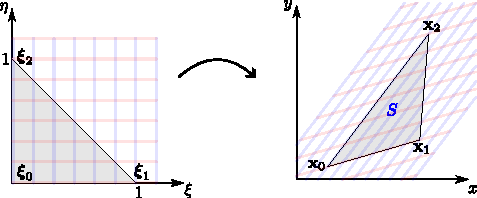
\includegraphics[width=0.6\linewidth]{lintri_transform.pdf}
\caption{Преобразование из параметрического треугольника}
\label{fig:lintri_transform}
\end{figure}
Рассмотрим двумерное преобразование, при котором
определяющие функции являются линейными. То есть представимыми в виде
\begin{align*}
x(\xi, \eta) = A_x \xi + B_x \eta + C_x, \\
y(\xi, \eta) = A_y \xi + B_y \eta + C_y.
\end{align*}
Для определения шести констант, определяющих это преобразование,
достаточно выбрать три любые (не лежащие на одной прямой) точки:
$(\xi_i, \eta_i) \to (x_i, y_i)$ для $i=0,1,2$.
В результате получим систему из шести линейных уравнений (три точки по две координаты),
из которой находятся конcтанты $A_{x,y}, B_{x,y}, C_{x,y}$.
Пусть три точки в параметрической плоскости
образуют единичный прямоугольный треугольник (\figref{fig:lintri_transform}):
\begin{equation*}
\xi_0, \eta_0 = (0, 0),\quad
\xi_1, \eta_1 = (1, 0),\quad
\xi_2, \eta_2 = (0, 1).
\end{equation*}
Тогда система линейных уравнений примет вид
\begin{align*}
&x_0 = C_x,       \quad y_0 = C_y, \\
&x_1 = A_x + C_x, \quad y_1 = A_y + C_y, \\
&y_2 = B_x + C_x, \quad y_2 = B_y + C_y.
\end{align*}
Определив коэффициенты преобразования их этой системы, окончательно запишем преобразование
\begin{equation}
\label{eq:lintri_transform}
\begin{aligned}
&x(\xi, \eta) = (x_1 - x_0)\xi + (x_2 - x_0) \eta + x_0,\\
&y(\xi, \eta) = (y_1 - y_0)\xi + (y_2 - y_0) \eta + y_0.\\
\end{aligned}
\end{equation}
Матрица Якоби этого преобразования \cref{eq:jacobi_matrix_2d}
не будет зависеть от параметрических координат $\xi, \eta$:
\begin{equation}
\label{eq:lintri_jacobi_matrix}
J = \left(
\begin{array}{cc}
x_1 - x_0 & x_2 - x_0 \\
y_1 - y_0 & y_2 - y_0 \\
\end{array}
\right).
\end{equation}
Якобиан преобразования будет равен удвоенной площади треугольника $S$, составленного из определяющих точек в физической плоскости:
\begin{equation}
\label{eq:lintri_jacobian}
|J| = (x_1 - x_0) (y_2 - y_0) - (y_1 - y_0) (x_2 - x_0) = (\vec x_1 - \vec x_0) \times (\vec x_2 - \vec x_0) = 2 |S|.
\end{equation}
Распишем интеграл по треугольнику $S$ по формуле \cref{eq:dxideta_integral}.
Вследствии линейности преобразования якобиан постоянен и, поэтому, его можно вынести его из-под интеграла:
\begin{equation}
\label{eq:lintri_integral}
\int\limits_{S}f(x, y)\,dxdy = |J|\int\limits_0^1 \int\limits_0^{1-\xi} f(\xi, \eta) d\eta d\xi.
\end{equation}

\subsubsubsection{Двумерное билинейное преобразование. Параметрический квадрат}
\label{sec:bilinquad_transform}
\begin{figure}[h!]
\centering
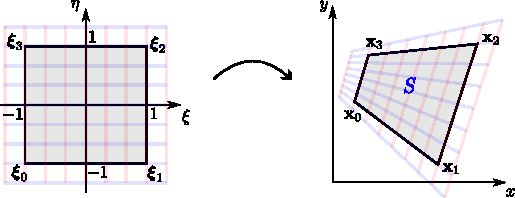
\includegraphics[width=0.6\linewidth]{bilinquad_transform.pdf}
\caption{Преобразование из параметрического квадрата}
\label{fig:bilinquad_transform}
\end{figure}

\subsubsubsection{Трёхмерное линейное преобразование. Параметрический тетраэдр}
TODO

\subsubsection{Свойства многоугольника}
\subsubsubsection{Площадь многоугольника}
\label{sec:polygon_area} 

\begin{figure}[h!]
\centering
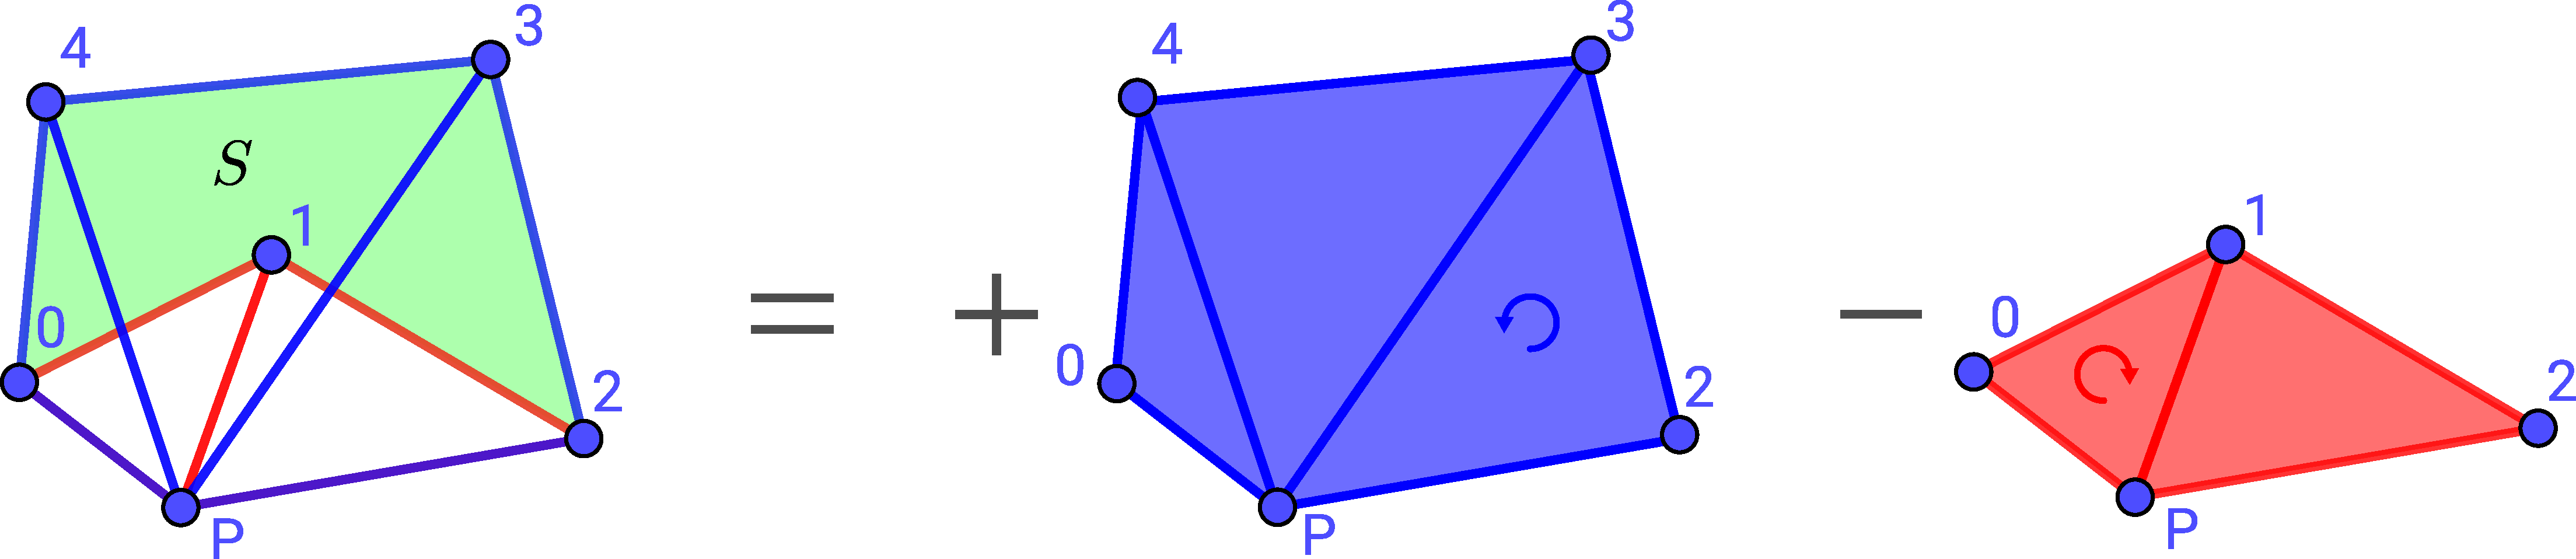
\includegraphics[width=0.7\linewidth]{polygon_area.pdf}
\caption{Площадь произвольного многоугольника}
\label{fig:polygon_area}
\end{figure}

Рассмотрим произвольный несамопересекающийся $N$-угольник $S$,
заданный координатами своих узлов $\vec x_i$, $i=\overline{0, N-1}$,
пронумерованных последовательно против часовой стрелки (\figref{fig:polygon_area}).
Далее введём произвольную точку $\vec p$ и 
от этой точки будем строить ориентированные треугольники до граней многоугольника:
$$
\triangle^p_i = (\vec p, \vec x_i, \vec x_{i+1}), \quad i=\overline{0, N-1},
$$
(для корректности записи будем считать, что $\vec x_N = \vec x_0$).
Тогда площадь исходного многоугольника $S$ будет равна сумме
знаковых площадей треугольников $\triangle^p_i$:
$$
|S| = \sum_{i=0}^{N-1} |\triangle^p_i|, \qquad |\triangle^p_i| = \frac{(\vec x_i - \vec p) \times (\vec x_{i+1} - \vec p)}{2}.
$$
Знак площади ориентированного треугольника зависит от направления закрутки его узлов:
она положительна для закрутки против часовой стрелки и отрицательна, если узлы пронумерованы по часовой стрелке.
В частности, на рисунке~\ref{fig:polygon_area} видно, что треугольники, отмеченные красным: $P01, P12$, будут
иметь отрицательную площадь, а синие треугольники $P23$, $P34$, $P40$ -- положительную. Сумма этих площадей
с учётом знака даст искомую площадь многоугольника.

Для сокращения вычислений воспользуемся произвольностью положения $\vec p$ и совместим
её с точкой $\vec x_0$. Тогда треугольники $\triangle^p_0$, $\triangle^p_{N-1}$
выродятся (будут иметь нулевую площадь).
Обозначим такую последовательную триангуляцию как
\begin{equation}
\label{eq:seq_polygon_triangulation}
\triangle_i = (\vec x_0, \vec x_i, \vec x_{i+1}), \qquad i=\overline{1,N-2}.
\end{equation}
Знаковая площадь ориентированного треугольника будет равна
\begin{equation}
\label{eq:seq_triangle_area}
|\triangle_i| = \frac{(\vec x_i - \vec x_0) \times (\vec x_{i+1} - \vec x_0)}{2}.
\end{equation}
Тогда окончательно формула определения площади примет вид
\begin{equation}
\label{eq:polygon_area}
|S| = \sum_{i=1}^{N-2}|\triangle_i|.
\end{equation}

\paragraph{Плоский полигон в пространтве} Если плоский полигон $S$ расположен в трёхмерном пространстве,
то правая часть формулы \cref{eq:seq_triangle_area} согласно определению векторного произведения в трёхмерном пространстве \cref{eq:vec_cross}
-- есть вектор.
Чтобы получить скалярную площадь, нужно спроецировать этот вектор на единичную нормаль к плоскости
многоугольника:
$$
\vec n = \frac{\vec k}{|\vec k|}, \qquad \vec k = (\vec x_1 - \vec x_0) \times (\vec x_2 - \vec x_0).
$$
Эта формула записана из предположения, что узел $\vec x_2$ не лежит
на одной прямой с узлами $\vec x_0$, $\vec x_1$. Иначе вместо $\vec x_2$ нужно
выбрать любой другой узел, удовлетворяющий этому условию.
Тогда площадь ориентированного треугольника, построенного
в трёхмерном пространстве запишется через смешанное произведение:
\begin{equation}
\label{eq:seq_triangle_area_3d}
|\triangle_i| = \frac{\left((\vec x_i - \vec x_0) \times (\vec x_{i+1} - \vec x_0) \right)\cdot \vec n}{2}.
\end{equation}
Формула для определения площади полигона \cref{eq:polygon_area} будет по прежнему верна.
При этом итоговый знак величины $S$ будет положительным,
если закрутка полигона положительная (против часовой стрелки) при взгляде со стороны
вычисленной нормали $\vec n$.

\subsubsubsection{Интеграл по многоугольнику}
\label{sec:polygon_integral} 
Рассмотрим интеграл функции $f(x,y)$ по $N$-угольнику $S$, заданному последовательными координатами своих узлов $\vec x_i$.
Введём последовательную триангуляцию согласно \cref{eq:seq_polygon_triangulation}.
Тогда интеграл по многоугольнику можно расписать как сумму интегралов по ориентированным треугольникам:
\begin{equation}
\label{eq:seq_triangulation_integral}
\arint{f(x,y)}{S}{xdy} = \sum_{i=1}^{N-2} \arint{f(x,y)}{\triangle_i}{xdy}.
\end{equation}
Далее для вычисления интегралов в правой части
воспользуемся преобразованием к параметрическому треугольнику (п.~\ref{sec:lintri_transform}).
Следуя формуле интегрирования \cref{eq:lintri_integral}, распишем
интеграл по $i$-ому треугольнику:
\begin{equation*}
\arint{f(x,y)}{\triangle_i}{xdy} = |J_i| \int\limits_{0}^{1}\int\limits_{0}^{1-\xi} f_i(\xi, \eta) \, d\eta d\xi,
\end{equation*}
где якобиан $|J_i|$ согласно \cref{eq:lintri_jacobian} есть удвоенная площадь ориентированного треугольника $\triangle_i$
(положительная при закрутке против часовой стрелке и отрицаетельная иначе):
\begin{equation*}
|J_i| = 2|\triangle_i| = (\vec x_i - \vec x_0) \times (\vec x_{i+1} - \vec x_0),
\end{equation*}
а функция $f_i(\xi, \eta)$ есть функция от преобразованных согласно \cref{eq:lintri_transform}
переменных:
\begin{equation*}
f_i(\xi, \eta) = f\left(\left(\vec x_i - \vec x_0\right)\xi + \left(\vec x_{i+1} - \vec x_0\right)\eta + \vec x_0\right).
\end{equation*}
Окончательно запишем
\begin{equation}
\label{eq:polygon_integral}
\arint{f(x,y)}{S}{xdy} = 2 \sum_{i=1}^{N-2}
    |\triangle_i| \int\limits_{0}^{1}\int\limits_{0}^{1-\xi} f_i(\xi, \eta) \, d\eta d\xi.
\end{equation}
Отметим, что эта формула работает и в том случае, когда
полигон расположен в трёхмерном пространстве
(знаковую площадь при этом следует вычислять по \cref{eq:seq_triangle_area_3d}).

\subsubsubsection{Центр масс многоугольника}
\label{sec:polygon_center} 
По определению, координаты центра масс $\vec c$ области $S$ равны среднеинтегральным значениям координатных функций. То есть
\begin{equation*}
c_x = \frac{1}{|S|}\int\limits_{S} x \, dxdy,
\quad 
c_y = \frac{1}{|S|}\int\limits_{S} y \, dxdy.
\end{equation*}
Далее распишем интеграл в правой части через последовательную триангуляцию согласно
\cref{eq:seq_triangulation_integral} с учётом линейного преобразования
\cref{eq:lintri_transform}:
\begin{align*}
\int\limits_{S} x \, dxdy &= \sum_{i=1}^{N-2} \int\limits_{\triangle_i} x \, dxdy\\
                          &= \sum_{i=1}^{N-2} |J_i| \int\limits_0^1\int\limits_0^{1-\xi} ((x_i - x_0)\xi + (x_{i+1} - x_0)\eta + x_0)\, d\eta d\xi\\
                          &= \sum_{i=1}^{N-2} \frac{|J_i|}{2}\frac{x_0 + x_i + x_{i+1}}{3}\\
                          &= \sum_{i=1}^{N-2} |\triangle_i|\frac{x_0 + x_i + x_{i+1}}{3}.
\end{align*}
Итого, с учётом \cref{eq:polygon_area}, координаты центра масс примут вид
\begin{align*}
&\vec c = \dfrac{\displaystyle\sum_{i=1}^{N-2} \dfrac{\vec x_0 + \vec x_i + \vec x_{i+1}}{3}|\triangle_i|}{\displaystyle\sum_{i=1}^{N-2} |\triangle_i|}.
\end{align*}
Если полигон расположен в двумерном пространстве $xy$, то знаковая площадь треугольников
вычисляется по формуле \cref{eq:seq_triangle_area}.
В случае трёхмерного пространтва должна использоваться формула \cref{eq:seq_triangle_area_3d}.

\subsubsection{Свойства многогранника}
\subsubsubsection{Объём многогранника}
\label{sec:polyhedron_volume} 
TODO
\subsubsubsection{Интеграл по многограннику}
\label{sec:polyhedron_integral} 
TODO
\subsubsubsection{Центр масс многогранника}
\label{sec:polyhedron_center} 
TODO

\subsubsection{Поиск многоугольника, содержащего заданную точку}
TODO


\section{Работа с инфраструктурой проекта CFDCourse}

\subsection{Сборка и запуск}
\subsubsection{Сборка проекта CFDCourse}

Описанная ниже процедура собирает проект в отладочной конфигурации.
Для проведения необходимых модификаций для сборки релизной версии смотри \ref{sec:release-build}.

\subsubsubsection{Подготовка}
\label{sec:install-prep}
\begin{enumerate}
\item
Для сборки проекта необходимо установить \ename{git} и \ename{cmake>=3.0}

В Windows необходимо скачать и установить диструбутивы:
\begin{itemize}
\item
\url{https://github.com/git-for-windows/git/releases/download/v2.43.0.windows.1/Git-2.43.0-64-bit.exe}
\item
\url{https://github.com/Kitware/CMake/releases/download/v3.28.3/cmake-3.28.3-windows-x86\_64.msi}
\end{itemize}

При установке cmake проследите, что бы путь к \ename{cmake.exe} сохранился в системных путях.
Msi установщик спросит об этом в диалоге.

В {\bf линуксе} используйте менеджеры пакетов, предоставляемые вашим дистрибутивом.
Также проследите чтобы были доступны компиллятор \ename{g++} и отладчик \ename{gdb}.

\item
Создайте папку в системе для репозиториев. Например \ename{D:/git_repos/}

\item
Возьмите необходимые заголовочные библиотеки boost из \url{https://disk.yandex.ru/d/GwTZUvfAqPsZBQ}
и распакуйте архив в папку для репозиториев (D:/git\_repos/boost).
Проследите, чтобы внутри папки boost сразу шли папки с кодом (\ename{accumulators}, \ename{algorithm}, ...)
и заголовочные файлы (\ename{align.hpp}, \ename{aligned_storage.hpp}, ...)
без дополнительных уровней вложения.

\item
Откройте терминал (git bash в Windows).

\item
С помощью команды cd в терминале перейдите в папку для репозиториев
\begin{shelloutput}
> cd D:/git_repos
\end{shelloutput}

\item
Клонируйте репозиторий
\begin{shelloutput}
> git clone https://github.com/kalininei/CFDCourse25
\end{shelloutput}
В директории (\ename{D:/git_repos} в примере) появится папка \ename{CFDCourse25}, которая является корневой папкой проекта
\end{enumerate}

\subsubsubsection{VisualStudio}
\label{sec:vs-build}

\begin{enumerate}
\item
Cоздайте папку build в корне проекта СFDCourse25

\item
Скопируйте скрипт winbuild64.bat в папку build. Далее вносить изменения
только в скопированном файле.

\item
Скрипт написан для версии \ename{Visual Studio 2019}. Если используется другая версия,
измените в скрипте значение переменной \cvar{CMGenerator} на соответствующие вашей версии.
Значения для разных версий Visual Studio написаны ниже
\begin{shelloutput}
SET CMGenerator="Visual Studio 17 2022"
SET CMGenerator="Visual Studio 16 2019"
SET CMGenerator="Visual Studio 15 2017"
SET CMGenerator="Visual Studio 14 2015"
\end{shelloutput}

\item
Запустите скрипт \ename{winbuild64.bat} из папки \ename{build}. Нужен доступ к интернету.
В процессе будет скачано около 200Мб пакетов, поэтому первый запуск может занять время

\item
После сборки в папке \ename{build} появится проект \ename{VisualStudio} \ename{cfdcourse25.sln}.
Его нужно открыть в \ename{VisualStudio}.
Дерево решения должно иметь следующий вид:
\begin{center}
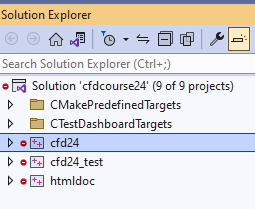
\includegraphics[width=0.3\linewidth]{vs_solution_explorer.png}
\end{center}
Проекты:
\begin{itemize}
\item \ename{cfd25} -- расчётная библиотека
\item \ename{cfd25_test} -- модульные тесты для расчётных функций
\end{itemize}

\item
Проект \ename{cfd25_test} необходимо назначить запускаемым проектом. Для этого нажать правой кнопкой мыши по проекту и в выпадающем меню
выбрать соответствующий пункт. После этого заголовок проекта должен стать жирным.
\begin{center}
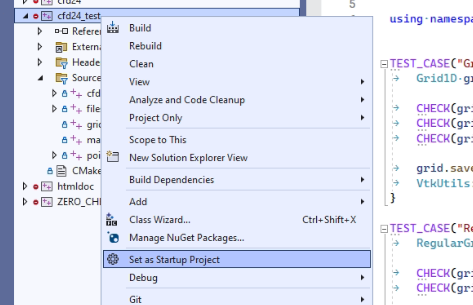
\includegraphics[width=0.5\linewidth]{win_startup_project.png}
\end{center}

\item
Скомпиллировать решение. Несколько способов:
\begin{itemize}
\item \ename{Ctrl+Shift+B},
\item \ename{Build->Build Solution} в основном меню,
\item \ename{Build Solution} в меню решения в дереве решения,
\item \ename{Build} в меню проекта \ename{cfd25_test}.
\end{itemize}

\item
Запустить тесты (проект \ename{cfd25_test}) нажав \ename{F5} (или кнопку отладки в меню).
После отработки должно высветиться сообщение об успешном прохождении всех тестов.

\item
Бинарные файлы будут скомпиллированы в папку \ename{CFDCourse25/build/bin/Debug}.
В случае работы через отладчик выходная директория, куда будут скидываться все файлы (в частности, vtk),
должна быть \ename{CFDCourse25/build/src/test/}.
\end{enumerate}

\subsubsubsection{VSCode}
\label{sec:vscode-build}

\begin{enumerate}
\item
Открыть корневую папку проека через \ename{File->Open Folder}
\item
Установить предлагаемые расширения cmake, c++
\item
Для настройки отладки создайте конфигурацию launch.json следующего вида
\begin{center}
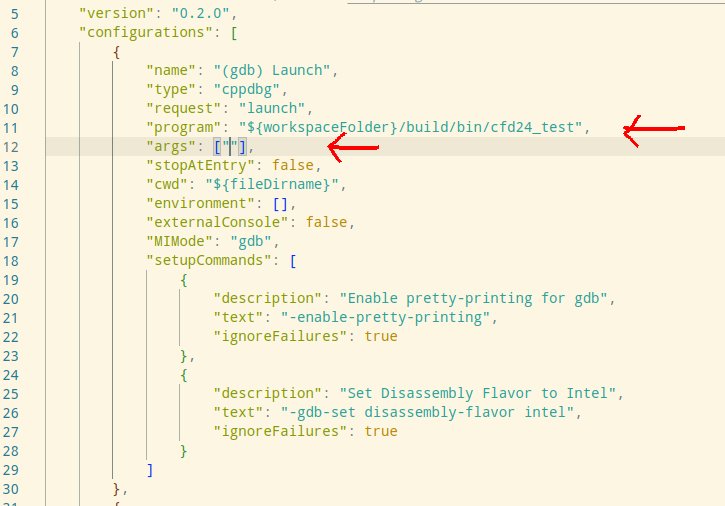
\includegraphics[width=0.7\linewidth]{vscode_launch_json.png}
\end{center}
\begin{itemize}
\item
Для этого перейдите в меню \ename{Run and Dubug} (\ename{Ctrl+Shift+D}), нажмите
\ename{create launch.json}, выберите пункт \ename{Node.js}.
\item
После этого в корневой папке появится файл \ename{.vscode/launch.json}.
\item
Откройте этот файл в \ename{vscode}, нажмите \ename{Add configuration}, \ename{(gdb) Launch} или \ename{(Windows) Launch} в зависимости от ОС.
\item
Далее напишите имя программы как показано на картинке.
\item
Используйте поле args для установки аргументов запуска.
\item
Выберите созданную конфигурацию для запуска отладчика по \ename{F5}
\begin{center}
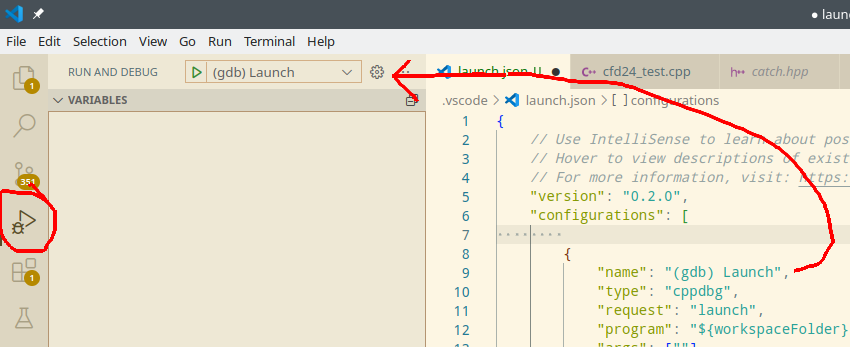
\includegraphics[width=0.7\linewidth]{vscode_launch.png}
\end{center}
\end{itemize}

На скриншотах представлены настройки в случае работы в линуксе. Для работы под виндоус 
\begin{shelloutput}
"name" : "(Windows) Launch",
"program": "${workspaceFolder}/build/bin/Debug/cfd25_test.exe"
\end{shelloutput}
\end{enumerate}

\subsubsection{Запуск конкретного теста}

По умолчанию программа \ename{cfd25_test} прогоняет все объявленные в проекте тесты. Иногда может возникнуть необходимость
запустить только конкретный тест в целях отладки или проверки.
Для этого нужно передать программе аргумент с тегом для этого теста.

Тег для теста -- это второй аргумент в макросе \cvar{TEST_CASE}, записанный в квадратных скобках.
Добавлять нужно вместе со скобками. Например, \cvar{[ping]}.

Чтобы добавить аргумент в \ename{VisualStudio}, необходимо в контекстном меню проекта \ename{cfd25_test} выбрать опции отладки
\begin{center}
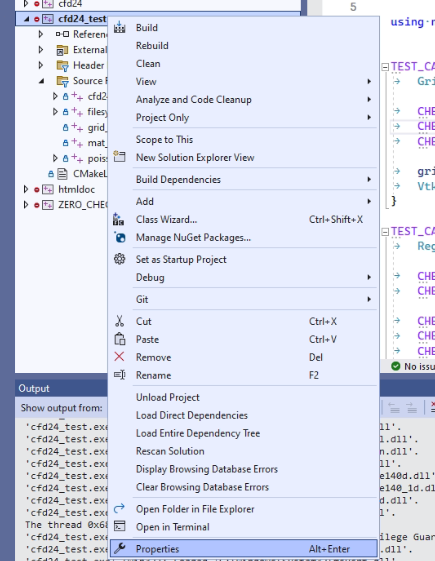
\includegraphics[width=0.7\linewidth]{win_debug_args_1.png}
\end{center}
и там в поле Аргументы прописать нужный тэг.
\begin{center}
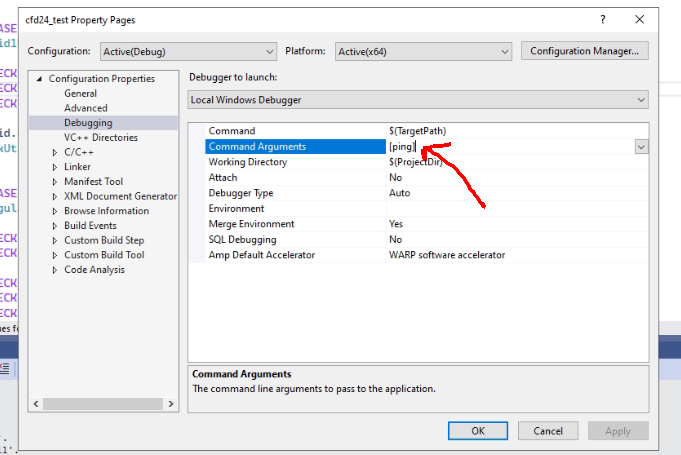
\includegraphics[width=0.9\linewidth]{win_debug_args_2.png}
\end{center}

В \ename{VSCode} аргументы нужно добавлять в файле \ename{.vscode/launch.json} в поле args в кавычках
(см. картинку \ref{sec:vscode-build} с настройками launch.json).

\subsubsection{Сборка релизной версии}
\label{sec:release-build}

Релизная сборка программ даёт многократное увеличение производительности,
но при этом отладка приложений в таком режиме невозможна.

{\bf Visual Studio}
\begin{enumerate}
\item Создать папку \ename{build-release} рядом с папкой \ename{build}.
\item Скопировать в неё файл \ename{winbuild64.bat} из папки \ename{build}. 
\item В скопированном файле произвести замену \cvar{Debug} на \cvar{Release}
\begin{shelloutput}
-DCMAKE_BUILD_TYPE=Release ..
\end{shelloutput}
\item Запустить \ename{winbuild64.bat} из новой папки
\item Открыть \ename{build-release/cfdcourse25.sln} в \ename{Visual Studio}
\item В проекте студии установить релизную сборку
\begin{center}
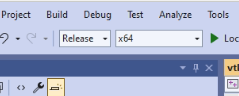
\includegraphics[width=0.5\linewidth]{release_build.png}
\end{center}
\item Это новое решение, не связанное настройками с \ename{debug}-версией.
      Поэтому нужно заново настроить запускускаемым проектом \ename{cfd_test}
      и, если нужно, настроить аргументы отладки.
\item Бинарные файлы будут скомпиллированы в папку \ename{CFDCourse25/build_release/bin/Release}.
      В случае работы через отладчик выходная директория -- \ename{CFDCourse25/build_release/src/test/}.
\end{enumerate}

{\bf VSCode}
\begin{enumerate}
\item Выбрать релизную сборку в \ename{build variant}
\item Нажать \ename{Build}
\item Нажать \ename{Launch}
\begin{center}
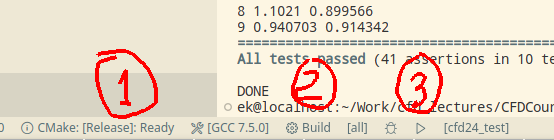
\includegraphics[width=0.5\linewidth]{release_build_2.png}
\end{center}
\end{enumerate}

\subsection{Git}
\subsubsection{Основные команды}
Все команды выполнять в терминале (\ename{git bash} для виндоус),
находясь в корневой папке проета CFDCourse24.
\begin{itemize}
\item
  Для {\bf смены директории} использовать команду \ename{cd}. Например, находясь в папке \ename{A} перейти в папку \ename{A/B/C}
  \begin{shelloutput}
> cd B/C
  \end{shelloutput}
\item
  {\bf Подняться} на директорию выше
  \begin{shelloutput}
> cd ..
  \end{shelloutput}
\item
  {\bf Просмотр статуса} текущего репозитория: текущую ветку, все изменённые файлы и т.п.
  \begin{shelloutput}
> git status
  \end{shelloutput}
\item
  {\bf Сохранить и скоммитить} изменения в текущую ветку
  \begin{shelloutput}
> git add .
> git commit -m "message"
  \end{shelloutput}

  ``message'' -- произвольная информация о текущем коммите, которая будет приписана к этому коммиту
\item
  {\bf Переключиться на ветку} main
  \begin{shelloutput}
> git checkout main
  \end{shelloutput}

  работает только в том случае, если все файлы скоммичены и статус ветки 'Up to date'
\item
  {\bf Создать новую ветку} ответвлённую от последнего коммита текущей ветки и переключиться на неё
  \begin{shelloutput}
> git checkout -b new-branch-name
  \end{shelloutput}

  new-branch-name -- имя новой ветки. Пробелы не допускаются

  Эта комманда работает даже если есть нескоммиченные изменения. 
  Если необходимо скоммитить изменеия в новую ветку, сразу за этой командой нужно вызвать
  \begin{shelloutput}
> git add .
> git commit -m "message"
  \end{shelloutput}
\item
  {\bf Сбросить} все нескоммиченные изменения. Вернуть файлы в состояние последнего коммита
  \begin{shelloutput}
> git reset --hard
  \end{shelloutput}

  Все изменения будут утеряны
\item
  {\bf Получить последние изменения} из удалённого хранилища с обновлением текущей ветки
  \begin{shelloutput}
> git pull
  \end{shelloutput}
  Работает только если статус текущей ветки 'Up to date'.\\
  Если требуется получить изменения, но не обновлять локальную ветку:
  \begin{shelloutput}
> git fetch
  \end{shelloutput}
  Обновленная ветка будет доступна по имени origin/{имя ветки}.
\item
  {\bf Просмотр истории} коммитов в текущей ветке (последний коммит будет наверху)
  \begin{shelloutput}
> git log
  \end{shelloutput}
\item
  {\bf Просмотр доступных веток} в текущем репозитории
  \begin{shelloutput}
> git branch
  \end{shelloutput}
\item
  {\bf Просмотр} актуального состояние дерева репозитория в gui режиме
  \begin{shelloutput}
> git gui
  \end{shelloutput}
  Далее в меню \ename{Repository->Visualize all branch history}.
  В этом же окне можно посмотреть изменения файлов по сравнению с последним коммитом.

  Альтернативно, при работе в виндоус можно установить программу GitExtensions и работать в ней.
\end{itemize}
  
\subsubsection{Порядок работы с репозиторием CFDCourse}

Основная ветка проекта -- \ename{main}. После каждой лекции (в течении 1-2 дней) в эту ветку будет отправлен коммит с сообщением \ename{after-lect{index}}.
Этот коммит будет содержать краткое содержание лекции,
задание по итогам лекции и необходимые для этого задания изменения кода.

Если предполагается работа с кодом на лекции, то перед лекцией в эту ветку будет отправлен коммит с сообщением \ename{before-lect{index}}.
Этот коммит содержит изменения кода для работы на лекции.

Таким образом, {\bf после лекции} необходимо выполнить следующие команды (находясь в ветке \ename{main})
\begin{shelloutput}
> git reset --hard  # очистить локальную копию от изменений,
                    # сделанных на лекции (если они не представляют ценности)
> git pull          # получить изменения
\end{shelloutput}

{\bf Перед началом лекции}, если была сделана какая то работа по заданиям,
\begin{shelloutput}
> git checkout -b work-lect{index}    # создать локальную ветку, содержащую задание
> git add .
> git commit -m "{свой комментарий}"  # скоммитить свои изменения в эту ветку
> git checkout main                   # вернуться на ветку main
> git pull                            # получить изменения
\end{shelloutput}

Даже если задание выполнено не до конца, вы в любой момент можете переключиться на ветку с заданием и его доделать
\begin{shelloutput}
> git checkout work-lect{index}
\end{shelloutput}

Если ничего не было сделано (или все изменения не представляют ценности), можно повторить алгоритм ``после лекции''.

\subsection{Paraview}

\subsubsection{Данные на одномерных сетках}
\label{sec:paraview-1d}

Заданные на сетке данные паравью показывает цветом.
Поэтому при загрузке одномерных сеток можно видеть картинку типа
\begin{center}
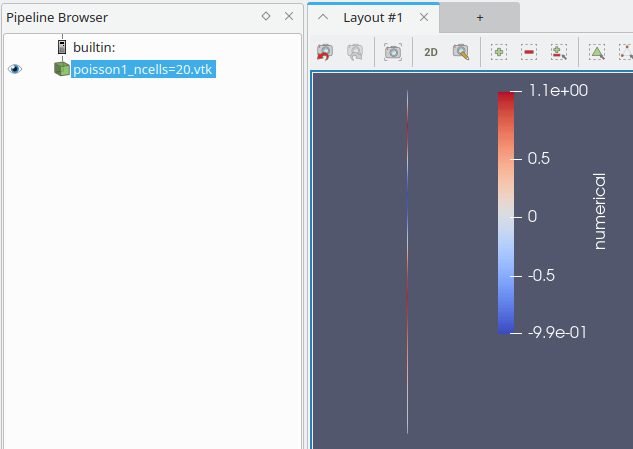
\includegraphics[width=0.5\linewidth]{howto_paraview_1d_1.png}
\end{center}
\paragraph{Развернуть изображение в плоскость xy}
\begin{center}
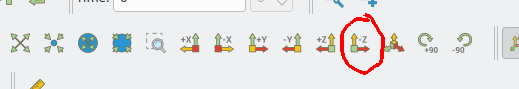
\includegraphics[width=0.5\linewidth]{howto_paraview_1d_2.png}
\end{center}
\paragraph{Отобразить данные в виде y-координаты} Для того, что бы данные отображались в качестве значения по оси ординат, к загруженному файлу необходимо
\begin{enumerate}
\item применить фильтр \ename{WarpByScalar} (В меню \ename{Filters->Alphabetical->Warp By Scalar})
\item в меню настройки фильтра указать поле данных, для отображения (numerical в примере ниже)
\item И настроить нормаль, вдоль которой будут проецироваться данные (в нашем случае ось y)
\end{enumerate}
\begin{center}
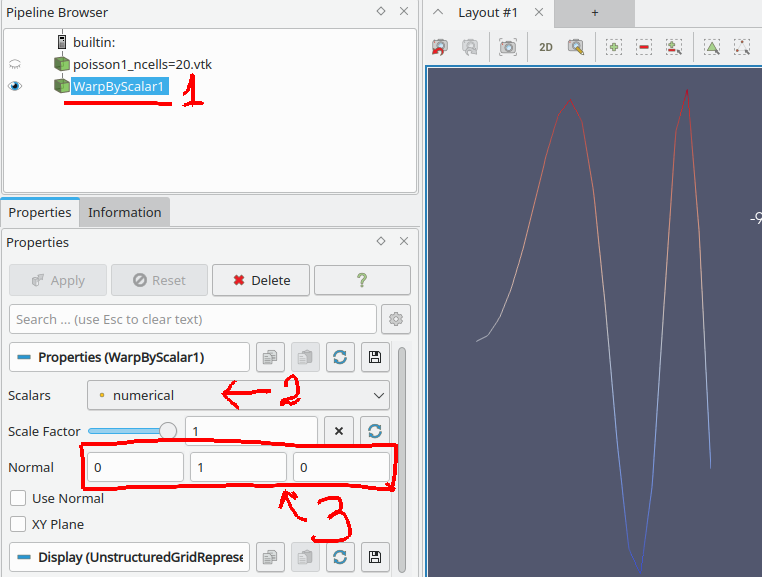
\includegraphics[width=0.5\linewidth]{howto_paraview_1d_3.png}
\end{center}

\paragraph{Цвет и толщина линии}
\begin{enumerate}
\item Включить подробные опции фильтра
\item Сменить стиль на \ename{Solid Color}
\item В меню \ename{Edit} выбрать желаемый цвет
\item В строке \ename{Line Width} указать толщину линии
\end{enumerate}
\begin{center}
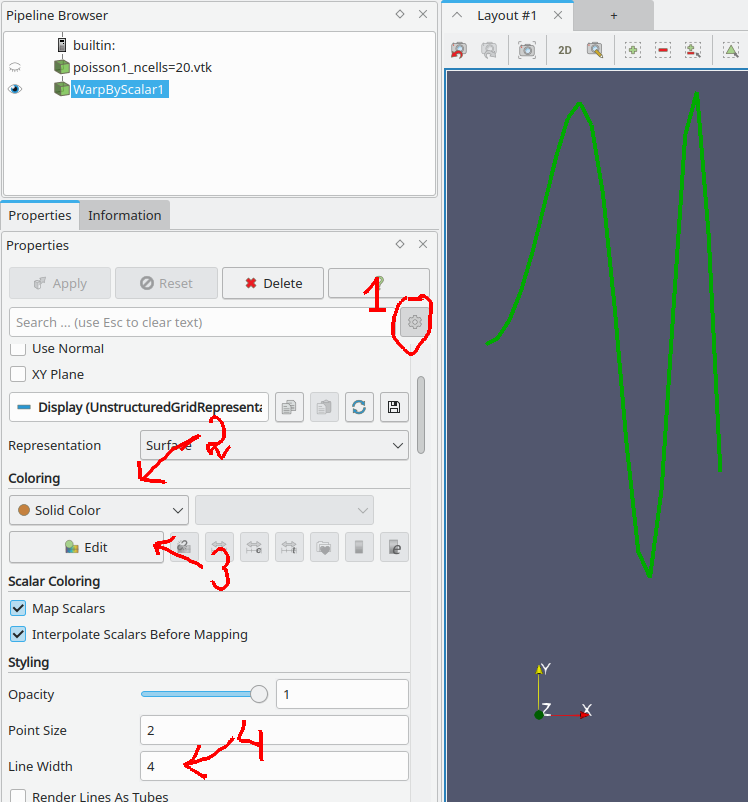
\includegraphics[width=0.6\linewidth]{howto_paraview_1d_4.png}
\end{center}

\paragraph{Настрока масштабов и отображение осей координат}
\begin{enumerate}
\item Отметье подробные настройки фильтра
\item В поле \ename{Transforming/Scale} Установите желаемые масштабы (в нашем случае растянуть в два раза по оси x)
\item Установите галку на отображение осей
\item откройте меню натройки осей
\item В нём включите подробные настроки
\item И также поставьте растяжение осей
\end{enumerate}
В случае, если масштабировать график не нужно, достаточно выполнить шаг 3.
\begin{center}
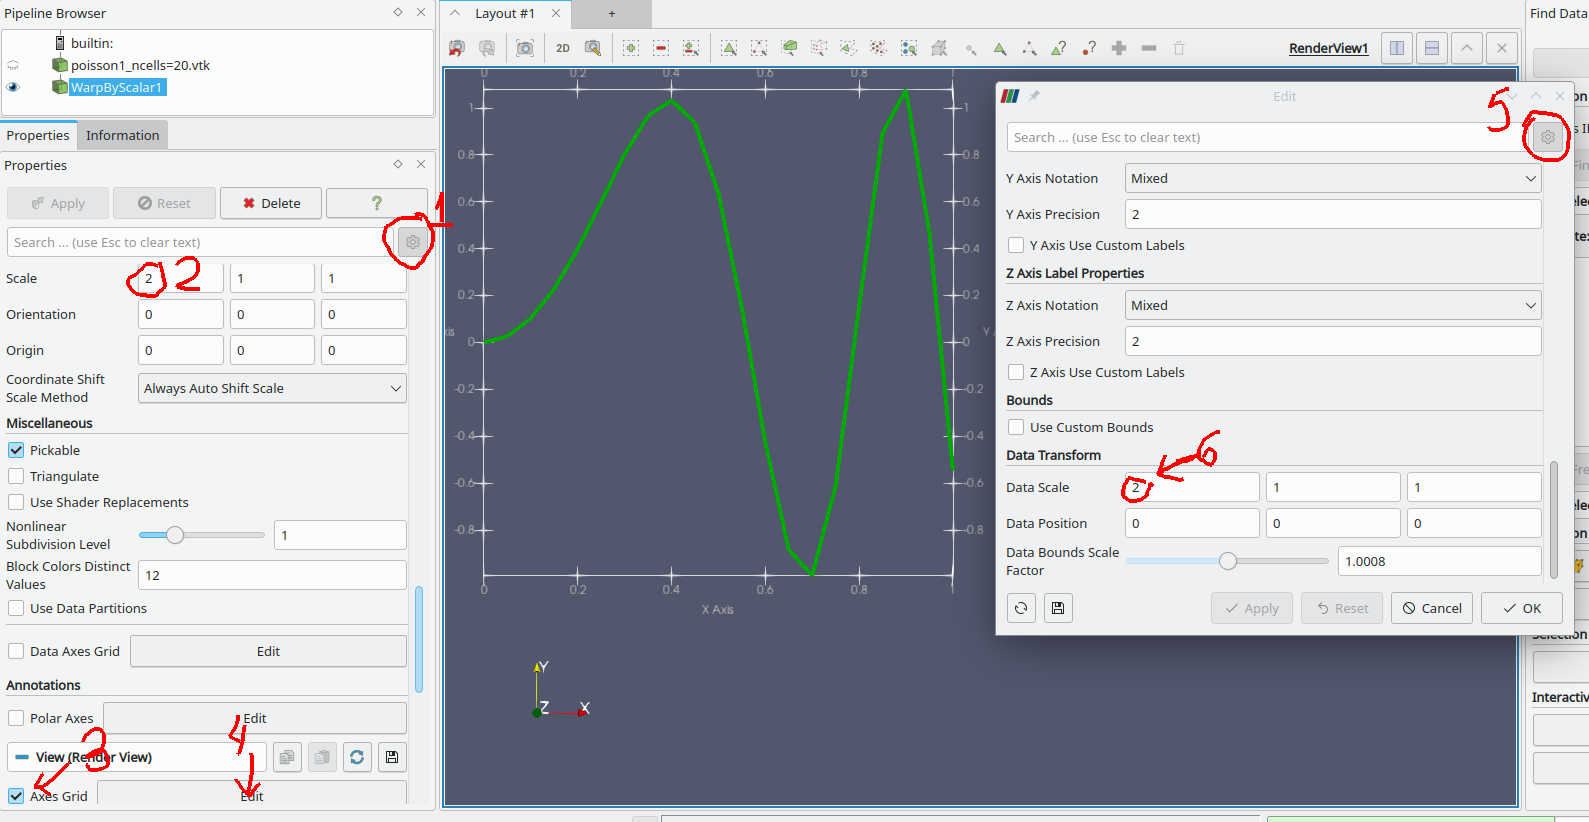
\includegraphics[width=0.9\linewidth]{howto_paraview_1d_5.png}
\end{center}

\paragraph{Построение графиков для нескольких данных}
Если требуется нарисовать рядом несколько графиков для разных данных из одного файла,
примените фильтр \ename{Warp By Scalar} для этого файла ещё раз, изменив поле \ename{Scalars} в настройке фильтра.
Для наглядности измените имя узла в Pipeline Browser на осмысленные
\begin{center}
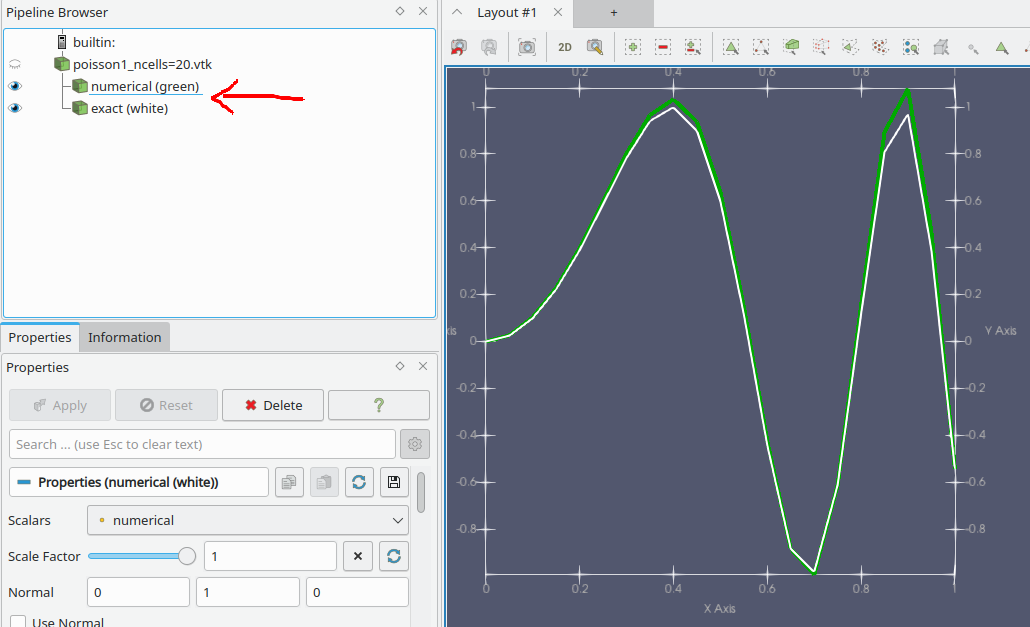
\includegraphics[width=0.8\linewidth]{howto_paraview_1d_6.png}
\end{center}

\paragraph{Обновление данных при изменении исходного файла}
В случае, если исходный файл был изменён, нужно в контекстном меню узла соответствующего файла
выбрать \ename{Reload Files} (или нажать F5). Если те же самые фильтры нужно применить для просмотра другого файла
нужно в этом меню нажать \ename{Change File}.
\begin{center}
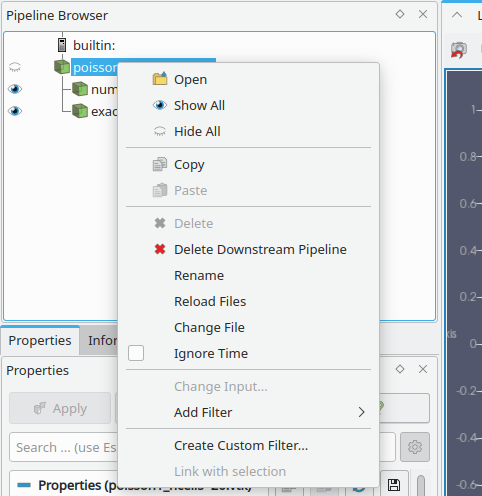
\includegraphics[width=0.4\linewidth]{howto_paraview_1d_7.png}
\end{center}

\subsubsection{Изолинии для двумерного поля}
\label{sec:paraview-isolines}

\begin{enumerate}
\item Нажмите иконку \ename{Contour} (или \ename{Filters/Contour})
      В настройках фильтра Contour by выберитее данные, по которым нужно строить изолинии.
\item В настройках фильтра удалите все существующие записи о значениях для изолиний
\item Добавьте равномерные значения. В появившемся меню установите необходимое количество изолиний и их диапазон.
\item Если необходимо, включите одновременное отображения цветного поля и изолиний.
\end{enumerate}

\begin{center}
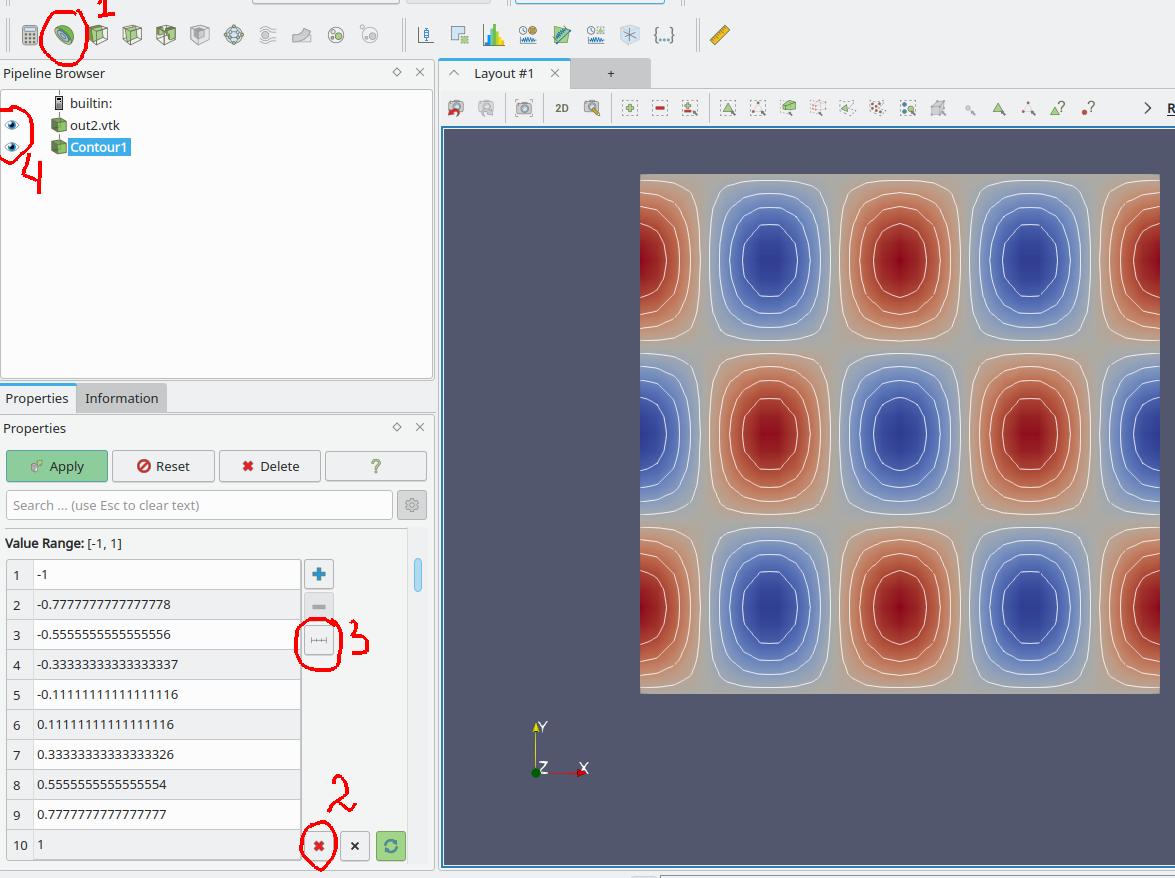
\includegraphics[width=0.7\linewidth]{howto_paraview_isolines_1.png}
\end{center}

\paragraph{Задание цвета и толщины изолинии}
В случае, если нужно сделать изолинии одного цвета, установите поле \ename{Coloring/Solid color} в 
настройках фильтра. Там же в меню \ename{Edit} можно выбрать цвет.
Для установления толщины линии включите подробные настройки и найдите там опцию \ename{Styling/Line Width}.
\begin{center}
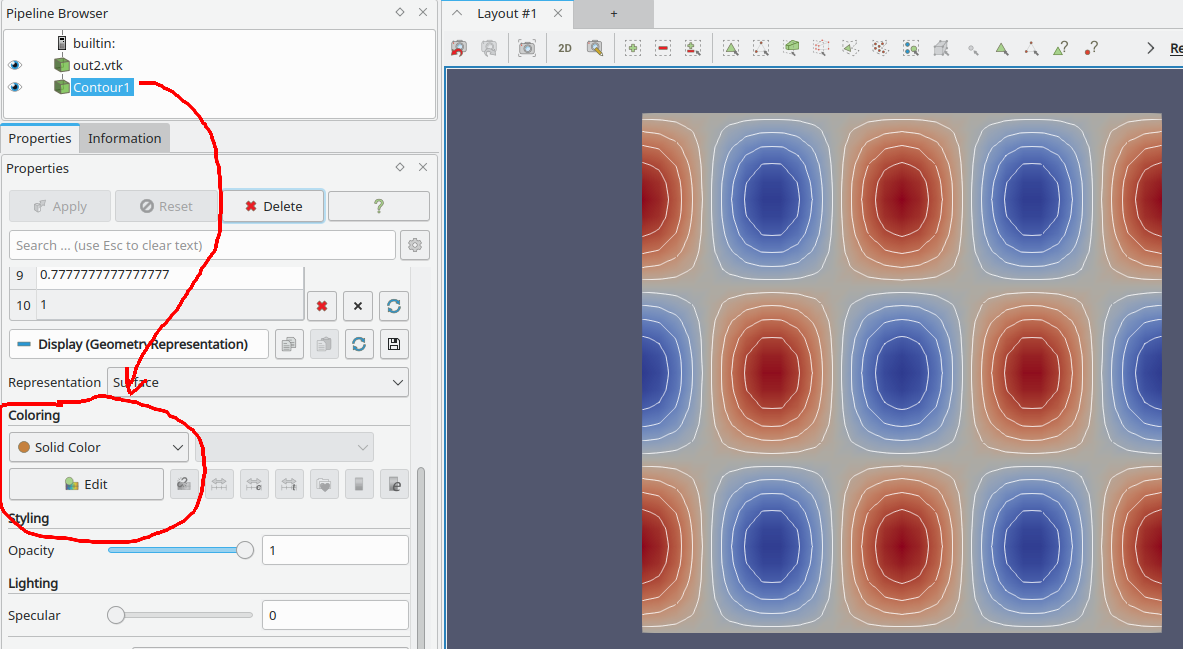
\includegraphics[width=0.7\linewidth]{howto_paraview_isolines_2.png}
\end{center}

\subsubsection{Данные на двумерных сетках в виде поверхности}
\label{sec:paraview-2d}

По аналогии с  одномерным графиком (п.~\ref{sec:paraview-1d}), двумерные поля так же
можно отобразить, проектируя данные на геометрическую координату для получения
объёмного графика. Для этого
\begin{enumerate}
\item Включите фильтр \ename{Filters/Warp By Scalar}
\item В настройках фильтра установите данные, которые будут проектироваться на координату z
\item Установите нормаль для проецирования (ось z)
\item Если нужно, выберите масштабирования для этой координаты
\item После нажатия \ename{Apply} включите трёхмерное отображение
\item Если данные не видно, обновите экран.
\end{enumerate}
\begin{center}
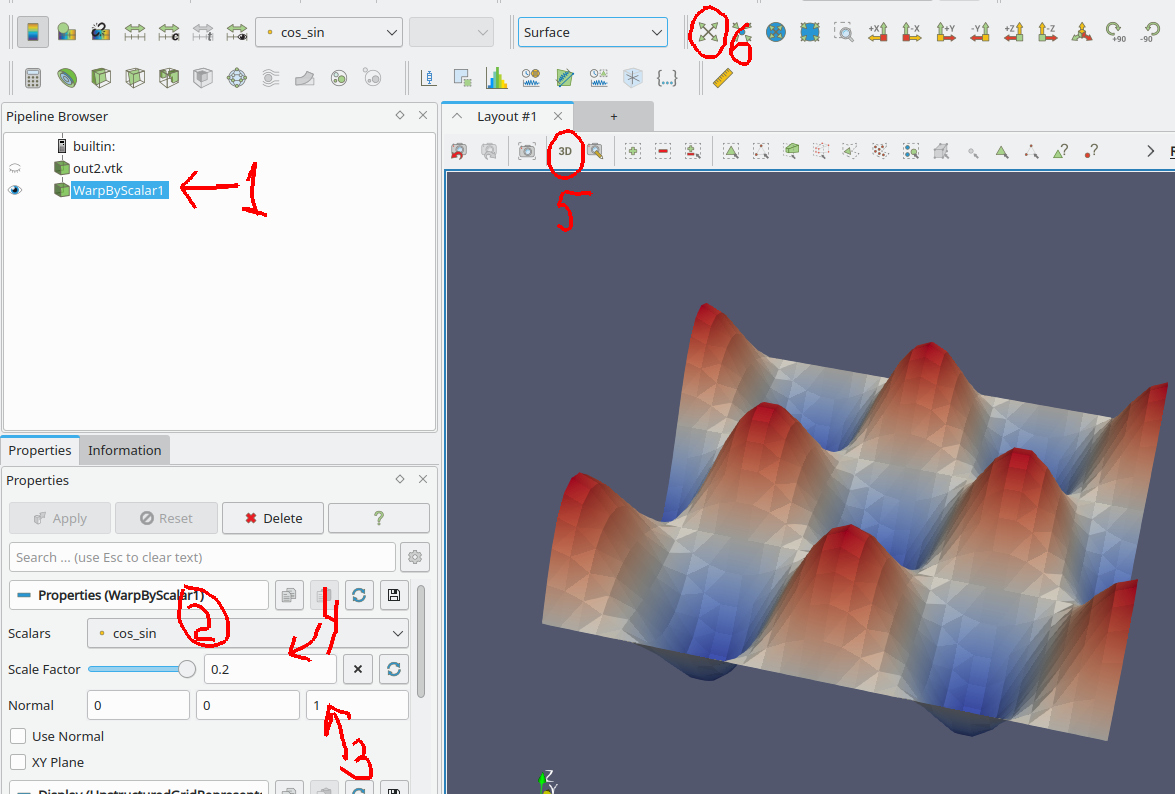
\includegraphics[width=0.9\linewidth]{howto_paraview_2d_as_3d.png}
\end{center}

\subsubsection{Числовых значения в точках и ячейках}
\label{sec:paraview-show-data}

Иногда в процессе отладки или анализа результатов расчёта
требуется знать точное значение поля в заданном узле или ячейке сетки.
Для этого

\begin{enumerate}
\item Включить режим выделения точек или ячеек (иконка (1 на рисунке) или горячие клавиши \ename{s}, \ename{d}).
      Выделить мышкой интересующую область
\item В окне \ename{Find data} (или \ename{Selection Inspector} для старых версий Paraview) отметить поле, которое должно отображаться 
      в центрах ячеек и в точках (2 на рисунке). Если такого окна нет, включить его из основного меню \ename{View}.
\end{enumerate}

\begin{center}
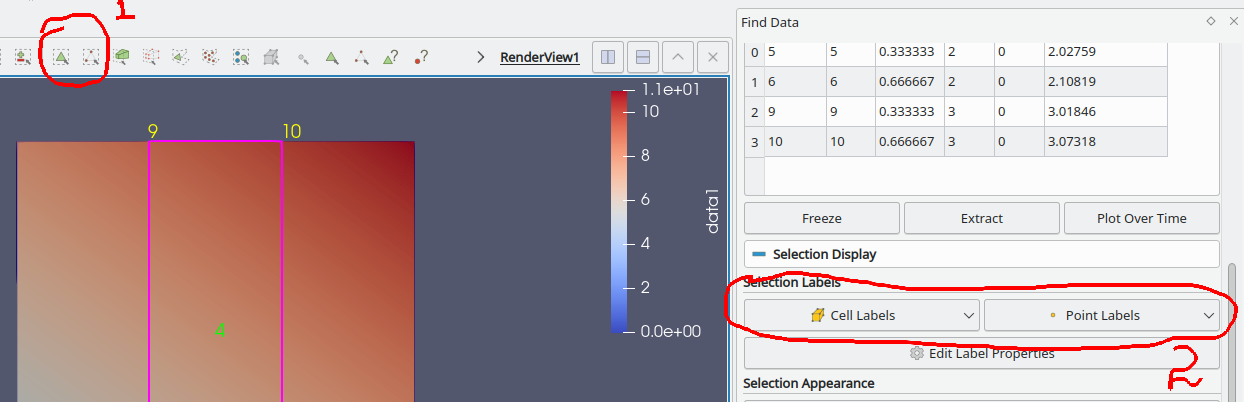
\includegraphics[width=0.8\linewidth]{howto_paraview_show_labels.png}
\end{center}

\subsubsection{Векторные поля}
\label{sec:paraview-glyph}

Открыть файл vtk или vtk.series, который содержит
векторное поле. Далее
\begin{enumerate}
\item Создать фильтр \ename{Glyph}
\item Задать двумерный тип стрелки
\item Сместить центр стрелки, чтобы она исходила из точки, к которой приписана
\item Отметить необходимое векторное поле в качестве ориентации
\item Отметить необходимое векторное поле для масштабирования
      Нажать \ename{Apply}.
\end{enumerate}

\begin{center}
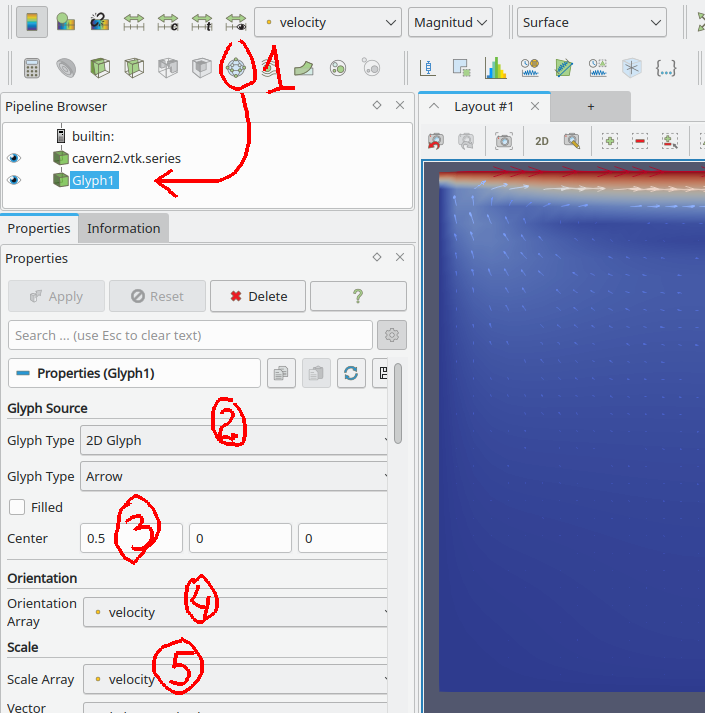
\includegraphics[width=0.6\linewidth]{glyph-1.png}
\end{center}

\paragraph{Настройка отображения стрелок}
\begin{enumerate}
\item Выбрать необходимый \ename{Glyph-mode}. Если сетка небольшая, то можно \ename{All Points}.
\item Установить белый цвет для стрелок. Нажать Apply.
\end{enumerate}

\begin{center}
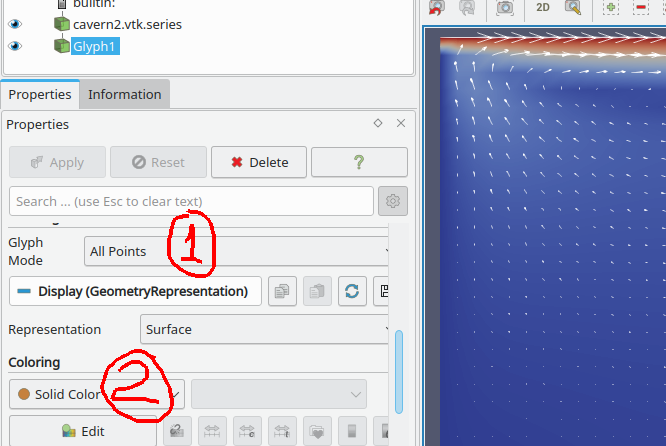
\includegraphics[width=0.4\linewidth]{glyph-2.png}
\end{center}

\paragraph{Уменьшения разброса по длине стрелок}
Если разброс по длинам стрелок слишком велик, его можно подравнять,
введя новую функцию $|\vec v|^{\alpha}$ -- длина вектора в степени меньше единицы (например, $\alpha=0.7$).
Такую функцию можно создать через калькулятор

\begin{enumerate}
\item Начиная от загруженного файла создать фильтр \ename{Calculator}
\item Там вбить необходимую формулу
\end{enumerate}
\begin{center}
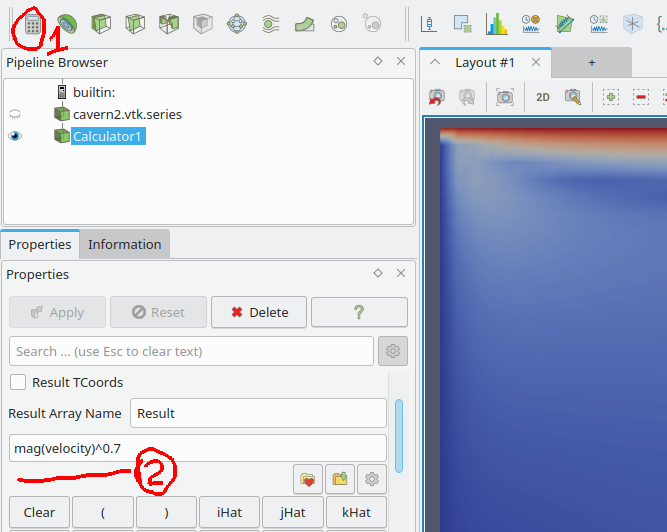
\includegraphics[width=0.6\linewidth]{glyph-3.png}
\end{center}
Созданную функцию нужно прокинуть в \ename{Glyph} в качестве коэффициента масштабирования
\begin{enumerate}
\item В \ename{Scale Array} фильтра \ename{Glyph} указать уже результат работы \ename{Calculator}-a (\ename{Result} по умолчанию),
\item Подтянуть значение \ename{Scale Factor} до приемлимого
\item Не забыть отключить вспомогательное поле \ename{Calculator} из отображения
\end{enumerate}
\begin{center}
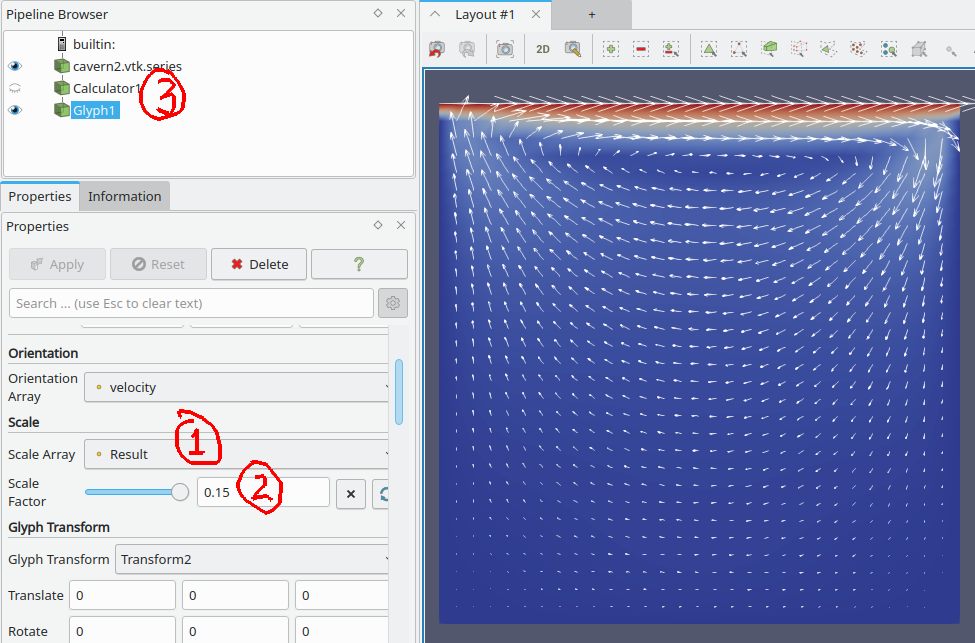
\includegraphics[width=0.6\linewidth]{glyph-4.png}
\end{center}

\subsubsection{Значение функции вдоль линии}
\label{sec:paraview-plot-over-line}

\begin{enumerate}
\item
Выбрать фильтр \ename{Plot Over Line} иконкой или в меню \ename{Filters}
\item
Установить начальную и конечную точку сечения
\item
Можно использовать привязку к узлам сетки с помощью горячих клавиш (в подсказках написано)
\item
Можно установить координаты руками в соответствующем поле. Для двумерных задач проследить,
что координата Z равна нулю
\item
Нажать \ename{Apply}
\end{enumerate}

\begin{center}
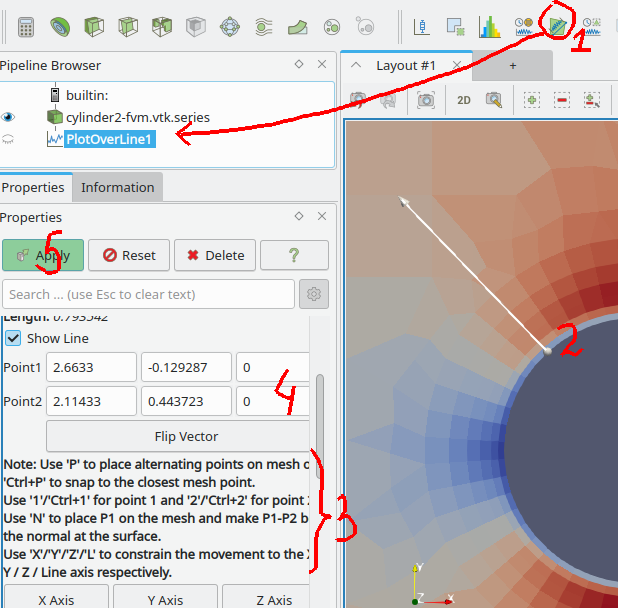
\includegraphics[width=0.4\linewidth]{howto_paraview_plot_over_line_1.png}
\end{center}

\paragraph{Настройка графика}
\begin{enumerate}
\item
После установок появится дополнительное окно типа \ename{Line Chart View} с нарисованным графиком.
\item
Сделав это окно активным в настройках фильтра \ename{PlotOverLine}
можно выбрать, какие поля рисовать (\ename{Series Parameters})
\end{enumerate}

\begin{center}
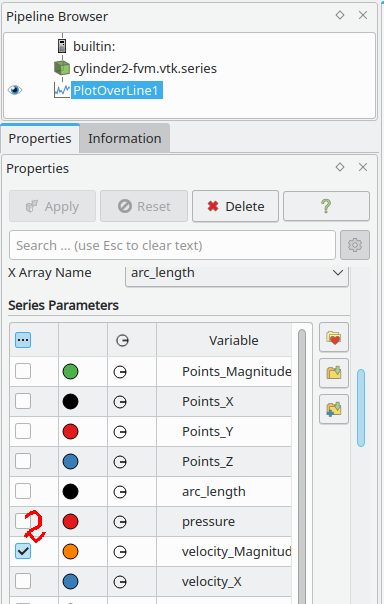
\includegraphics[width=0.2\linewidth]{howto_paraview_plot_over_line_3.png}
\quad
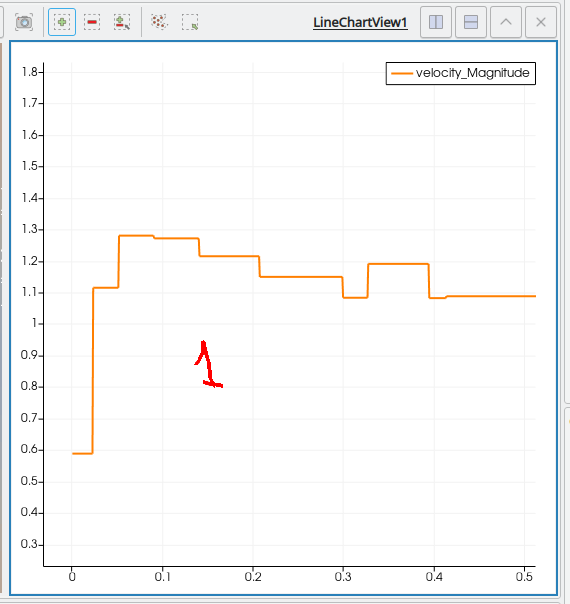
\includegraphics[width=0.3\linewidth]{howto_paraview_plot_over_line_2.png}
\end{center}

\paragraph{Отрисовка в отдельном окне}
\begin{enumerate}
\item
Открыть новую вкладку
\item
Выбрать \ename{Line Chart View}
\item
Выбрать предварительно созданный фильтр с одномерным графиком
\end{enumerate}
\begin{center}
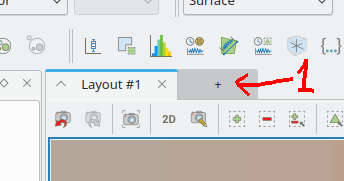
\includegraphics[width=0.2\linewidth]{howto_paraview_plot_over_line_4.png}
\quad
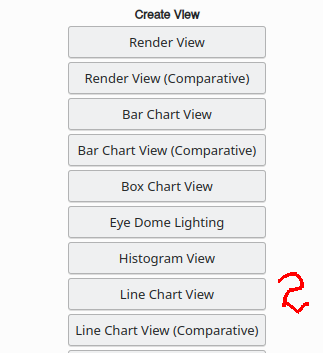
\includegraphics[width=0.3\linewidth]{howto_paraview_plot_over_line_5.png}
\quad
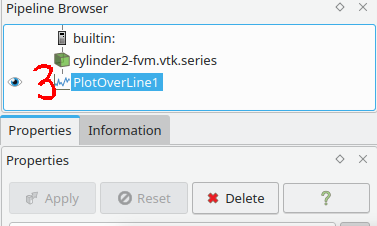
\includegraphics[width=0.3\linewidth]{howto_paraview_plot_over_line_6.png}
\end{center}

\subsection{Hybmesh}
\label{sec:hybmesh}

Генератор сеток на основе композитного подхода.
Работает на основе python-скрипотов.
Полная документация \url{http://kalininei.github.io/HybMesh/index.html}

\subsubsection{Работа в Windows}
Инсталлятор программы следует скачать по ссылке
\url{https://github.com/kalininei/HybMesh/releases}
и установить стандартным образом.

Для запуска скрипта построения \ename{script.py} нужно
открыть консоль, перейти в папку с нужным скриптом,
оттуда выполнить (при условии, что программа была установлена в папку \ename{C:\Program Files}):
\begin{shelloutput}
> "C:\Program Files\HybMesh\bin\hybmesh.exe" -sx script.py
\end{shelloutput}

\subsubsection{Работа в Linux}
Версию для линукса нужно собирать из исходников.
Либо, если собрать не получилось,
можно строить сетки в Windows и переносить
полученные vtk-файлы на рабочую систему. 

Перед сборкой в систему необходимо установить dev-версии
пакетов \ename{suitesparse} и \ename{libxml2}. Также 
должны быть доступны компилляторы \ename{gcc-c++} и \ename{gcc-fortan} и \ename{cmake}.
Программа работает со скиптами python2.
Лучше установить среду anaconda (\url{https://docs.anaconda.com/free/anaconda/install/index.html})
И в ней создать окружение c python-2.7:
\begin{shelloutput}
> conda create -n py27 python=2.7   # создать среду с именем py27
> conda activate py27               # активировать среду py27
> pip install decorator             # установить пакет decorator
\end{shelloutput}

Сначала следует склонировать репозиторий в папку с репозиториями гита:
\begin{shelloutput}
> cd D:/git_repos
> git clone https://github.com/kalininei/HybMesh
\end{shelloutput}

Поскольку программа не предназначена для запуска из под анаконды,
в сборочные скрипты нужно внести некоторые изменения.
В корневом сборочном файле \ename{HybMesh/CMakeLists.txt} 
нужно закомментировать все строки в диапазоне
\begin{minted}[linenos=false]{text}
# ========================== Python check
....
# ========================== Windows installer options
\end{minted}
а в файле \ename{HybMesh/src/CMakeLists.txt} последнюю строку
\begin{minted}[linenos=false]{text}
#add_subdirectory(bindings)
\end{minted}

Далее, находясь в корневой директории репозитория HybMesh, запустить сборку
\begin{shelloutput}
> mkdir build
> cd build
> cmake .. -DCMAKE_BUILD_TYPE=Release
> make -j8
> sudo make install
\end{shelloutput}

Для запуска скриптов нужно создать скрипт-прокладку
\begin{minted}[linenos=false]{python}
import sys
sys.path.append("/path/to/HybMesh/src/py/")  # вставить полный путь к Hybmesh/src/py
execfile(sys.argv[1])
\end{minted}
и сохранить его в любое место. Например в \ename{path/to/HybMesh/hybmesh.py}.

Для запуска скрипта построения сетки следует перейти в папку, где находится нужный скрипт \ename{script.py},
убедится, что анаконда работает в нужной среде (то есть \ename{conda activate py27} был вызван),
и запустить
\begin{shelloutput}
> python /path/to/HybMesh/hybmesh.py script.py
\end{shelloutput}


\end{document}
